\chapter[Encoding language]{Encoding language on computers}
\label{ch:encodings}

\section{What is language?}

This book aims to introduce you to the different ways that computers are able to process natural language.  To start off, then, we can ask: What is language?  You're using language to read this book, so you have some intuitive idea of what it is, but if you've never studied linguistics before, you might not have a clear definition in mind.

In an attempt to distinguish between language and other animal communication systems, the anthropologist  Charles \citet{Hockett:1960}  proposed some properties that together make language special:

\begin{enumerate}
    \item Language is produced vocally and understood with the auditory system, or in the case of signed languages, signed with the body and perceived visually.
    \item Language is produced intentionally. People intend to say what they say.
    \item Language is transitory: Unless you write down what is said, it is ephemeral.  As we will explore in detail later, writing -- crucially \emph{not} transitory -- is distinct from language.
    \item Language is interchangeable: Anything that you can hear, you can also say, and vice versa, regardless of its truth or its relation to you. (In contrast, in the realm of animal communication, queen ants produce a chemical signal that other ants cannot produce, meaning that chemical communication for ants is non-interchangeable.)
    \item Language involves total feedback: Speakers can hear their own speech, and signers can see their own signing.  People know what they are saying.
    \item When people speak or sign, the sounds/signs that they produce are specifically intended for communication, not secondary to any other purpose.  (In contrast, a dog may indirectly convey that it is hot by panting, but the primary purpose of panting is to cool the dog off, not to communicate.)
    \item Specific words/signs are attached to specific meanings.
    \item The relation between sounds/signs and meaning is mostly \keyword{arbitrary}, chosen by convention.  There is no particular reason to call a dog a \exword{dog} except that our community has agreed to it; other communities have chosen other conventions (\exword{perro}, \exword{Hund}, etc.).
    \item Even if different people pronounce or sign the same word differently, these  variable realizations are mapped to discrete categories (distinct sounds, signs, or words) in the mind.
    \item Language can be used to talk about things that are absent, imaginary, or false (in contrast to pointing, for example, which is restricted to entities that are present).
    \item Language can be used to lie.
    \item Language is made of discrete units: Sentences/utterances are made of words; words are made of morphemes (pieces of words such as \exword{un-} or \exword{-ing}); morphemes are made of sounds.
    \item Language is \keyword{productive}: You can use it to say and understand things that have never been said before.
    \item Language is learnable: You can learn a (new) language.
    \item Language is culturally transmitted: You learn the
      language(s) surrounding you.
    \item Language is reflexive: As we're doing here, you can use language to talk about itself.

\end{enumerate}

Using these distinctive features, you should now be able to explain why music, mathematics, and programming languages -- as amazing and useful as they are -- do not constitute language in Hockett's sense, even if they share some elements in common with it.

\section{Language versus writing}

Language is perhaps the most amazing technology that humans have ever created: It allows us to teach and learn,  explain complicated ideas,  build social relationships and societies,  create laws and promises,  ask and answer questions, make and respond to commands, tell stories, imagine alternate realities, understand what other people believe,  recount the past and plan for the future, and  collaborate to get things done.


It is important to understand that language is distinct from writing.  As Hockett notes, spoken/signed utterances are ephemeral; writing constitutes a further amazing technology which represents speech/signing in a system of lasting physical or digital markings.
 Distinguishing language from its written representation,  language is universal across humans: All human societies use language, and every single human child (except for rare cases of extremely severe neglect or disability) learns language without much formal instruction.  In contrast, writing is not universal: Some societies do not use writing.  Indeed, of the seven thousand known spoken languages listed in  \mediatitle{Ethnologue}\footnote{\url{https://ethnologue.com}, accessed 2024-04-19.}, only about sixty percent have writing systems; unwritten languages include the  Gugu Badhun language of Australia, the Southeastern Pomo language of California, and so on. 
Writing generally requires formal instruction, and some people do not learn it even if their society uses it.  Language is also much older than writing; language emerged around 100,000 to 200,000 years ago while writing arose around five or six thousand years ago.  Of course, language is transitory, so its age can only be inferred indirectly, from archaeological artifacts such as decorative beads \citep{BothaKnight:2009}, which indicate a desire to communicate (one's status and appearance) that presumably extends to language. So language is ancient and universal, while writing is new and localized to particular people and societies.

Although it is important to keep language and writing distinct, writing is obviously intimately related to language.  Writing  allows us to do all the things that language allows us to do -- teach, learn, explain, build relationships, organize societies, talk about the past and future, collaborate -- across distances and time.  With writing, you can learn from people you have never met, from past generations and other continents.  You can also keep records of things, such as debts and purchases, that are too complicated to remember; 
%\mad{Do we have a reference or further reading for this? $\to$ Lelia} \faye{Glassner's book "The Invention of Cuneiform" (2003) could be valuable additional reading here?}
indeed, the first Sumerian writing appears to record commercial transactions, involving both language and numeracy  \citep{Glassner:2003}.  Today, thanks to computers and the internet, digital writing allows us to disseminate language instantly around the globe.

The topics explored in this book involve the word \exword{language} -- natural language processing, language technology -- but they largely involve writing, because writing is the primary medium through which computers represent and process language.  We begin our tour by introducing writing systems and their digital representation, then end the chapter by briefly exploring sound.

%Even \keyword{dialog systems} such as Siri and Google Home, which interpret and produce speech, map that speech to text and then to speech again.  Speech/signing is transitory and fades quickly from a listener's memory, whereas writing is sufficiently permanent that it can be manipulated digitally.\wdm{This may come across as a bit simplistic since it \textbf{is} possible to encode spoken language so that it is as permanent as writing. And,  a transcription of speech is not the same as a written text. So should we soften this and reformulate it to be a transition to both writing systems (the next section) and encoding spoken language (coming up in 1.5?) $\to$ Detmar} 





% It's  late 

%As but one example, think about what happens when a friend points at a book and says, \exsent{He's no Shakespeare!}.  First of all, there is the difficulty of determining who is meant by \exsent{he}.  Your friend is pointing at a book, not at a person, and although we can figure out that \exsent{he} most likely refers to the author of the book, this is not obvious to a computer (and sometimes not obvious to the person you are talking with).  Secondly, there is the difficulty of knowing who \exsent{Shakespeare} is.  Shakespeare is the most famous writer in the English language, but how does a computer know that?  Or, what if your friend had said \exsent{He's no Lessing!}?   English majors with an interest in science-fiction or progressive politics might take  this as a reference to Doris Lessing,  students of German literature might suspect a comparison to G.E. Lessing, the elegant Enlightenment stylist of German theater, but in the absence of background knowledge, it is hard to know what to make of this remark.

%Finally, even if we unpack everything else, consider what your friend's statement literally means: the author of this book is not William Shakespeare.   Unless there is a serious possibility that the book \emph{was} written by Shakespeare, this literal meaning is a such a crushingly obvious truth that it is difficult to see why anyone would bother to express it.  In context, however, we can tell that your friend is not intending to express the literal meaning, but  rather to provide a negative evaluation of the author relative to Shakespeare,  who is the standard benchmark for good writing in English.  You could do the same thing for a slim book of mystical poetry by saying \exsent{She's no Dickinson},  provided the hearer was going to understand that the reference was to Emily.

%Or consider a different kind of statement: \exsent{I'm going to the   bank with a fishing pole}.  Most likely, this means that the speaker is going to a river bank and is carrying a fishing pole.  But it could also mean that the speaker is going to a financial institution, carrying a fishing pole, or it could mean that the speaker is going to a financial institution known for its fishing pole -- or even that the river bank the speaker is going to has some sort of notable fishing pole on it.  


\section{Writing systems}


A \keyword{writing system} is ``a system of more or less permanent marks used to represent an utterance in such a way that it can be
recovered more or less exactly without the intervention of the utterer'' \citep[3]{daniels:bright:96}.   %Writing allows us to communicate with people (including ourselves) across time and space, preserving and disseminating ideas in ways not otherwise possible.  
Historically, of course, writing systems consisted of markings on clay, stone, or paper (originally made by hand, later by the printing press); today, these markings are  stored and disseminated digitally, allowing for much more text to be written, read, and shared than at any other time in history.


You are reading this book in the Latin alphabet: 26 letters, each of which has an upper-case and a lower-case variant, plus ten numerals and various types of punctuation: In total, a little over a hundred symbols.  Simple enough?

But this book is called \emph{Language and computers}, not \emph{English and computers}!  So we also have to think about how to represent other languages and other writing systems.


First, going back to the idea that writing systems are distinct from languages, many different languages share the same writing system: The Latin alphabet is used not just for English but also for French, German, Finnish,  Vietnamese, Yoruba, and many other languages.  


\ea   Same writing system, different languages:
\ea   English: What is your name? 
\ex   French: \exsent{Comment t'appelles-tu?}
\z 
\z 
 
Conversely, the same language can be written in multiple different writing systems.  Mandarin Chinese can be written in the traditional characters still used today in Taiwan; in the simplified characters of Mainland China; or transliterated into the Latin alphabet through the Pinyin system.  

\begin{figure}
    \begin{tabular}{ccc}
      
\includegraphics[width=.05\textwidth]{figures/05-chinese-kaishu-trad} &
      
\includegraphics[width=.05\textwidth]{figures/06-chinese-simplified.jpg} & 
            \Large{m\v{a}}  \\

       Traditional character & Simplified character & Pinyin Latinization \\ 
    \end{tabular}
    \caption{`Horse' (\exword{m\v{a}}) written in three different writing systems for Mandarin Chinese.}
    \label{fig:samelg:diffwriting}
\end{figure}


As another example of how languages are distinct from writing systems, Yiddish and German are related to one another and somewhat mutually intelligible, but German is written in the Latin alphabet while Yiddish is written in the Hebrew writing system (which, as we'll discuss below, is not a traditional alphabet because only the consonant sounds are written).

Turkish and Vietnamese are examples of languages  currently written in the Latin alphabet but which historically used other systems (for Turkish, Arabic and Greek alphabets; for Vietnamese, an adaption of the Chinese writing system).   Japanese is a single language currently written in three different writing systems, all of which can be used for different purposes within the same document.  %Kanji characters, borrowed from the Chinese writing system, represent meaning rather than sound and were historically used by the most educated people.  Katakana represents syllables phonetically and is used to write foreign words and sometimes as a substitute for kanji.   Hiragana, which also represents syllables phonetically, is used most widely. 


As discussed above, language comprises a set of mostly arbitrary, memorized pairs of sound and meaning.  A writing system can in principle reflect either or both of these elements, sounds or meaning.  We will explore three types of writing systems: alphabetic (where each symbol represents one sound), syllabic (each symbol represents a syllable), and logographic (each symbol represents a concept that language refers to). 
In any such system, some part of the sound/meaning pairing is recorded, but other parts must be independently known to the reader.  Reading English in the Latin alphabet, the string of letters \textit{cat} conveys information about pronunciation, but you have to already know the meaning associated with this string of sounds.

Writing systems vary not just in what information is or is not encoded, but also in their direction (the Latin alphabet is conventionally written left to right; the Hebrew and Arabic systems go right to left; Chinese used to be written vertically but is now written left to right); in conventions about capitalization (if it exists) and punctuation; and in whether words or syllables are separated (in the Latin alphabet, by spaces) or contiguous.





%For writing English, the idea is that each letter should correspond to an individual sound, more or less, but this need not be so (and it is not entirely true in English).  Each character could correspond to a series of sounds (e.g., a single character for \exword{str}), but we could also go in a different direction and have characters refer to meanings.  Thus, we could have a character which stands for the meaning of \exsent{dog}.  Types of writing systems vary in how many sounds a character represents or to what extent a meaning is captured by a character.  Furthermore, writing system differ in whether they even indicate what a word is, as English mostly does by including spaces; we will return to this issue of distinguishing words in chapter~\ref{sec:adding-linguistic-analysis}.



\subsection{Alphabetic systems}
\label{sec:alpha}

We start our tour of writing systems with what should be familiar to
any reader of English: \keywordAs{alphabets}{alphabet}.  In \keywordAs{alphabetic systems}{alphabetic system}, a
single character typically refers to a single sound (a single articulatory gesture made by the vocal apparatus).  In the word \exword{cat}, the three letters represent three sounds: an initial consonant, a vowel, and a final consonant.

But there is not always a perfect one-to-one correspondence between a word's alphabetic
spelling and its pronunciation.  In English,  the orthographic
string \exword{ough} can be pronounced at least five
different ways: \exword{c\uline{ough}}, \exword{t\uline{ough}}, \exword{thr\uline{ough}}, \exword{th\uline{ough}}, and
\exword{hicc\uline{ough}}.  Letters
are not consistently pronounced, and in fact, sometimes they are not
pronounced at all, as in   in \exword{\uline{k}nee},
\exword{de\uline{b}t}, \exword{\uline{p}sychology}, and \exword{mor\uline{t}gage}, among others.  There
are historical reasons for these silent letters, which were by and
large pronounced at one time, but the effect is that we now have
letters we do not speak.

The idealized one-to-one sound-letter correspondence is also disrupted when single letters  represent
multiple sounds, such as the \exword{x} in \exword{ta\uline{x}}, which
corresponds to a [k] sound followed by an [s] sound.
Moreover, multiple letters can consistently be used to represent one sound,
as in  \exword{sh} in \exword{\uline{sh}ould} or  \exword{ti} in
\exword{revolu\uline{ti}on} -- both of which represent a single articulatory gesture in which air is channeled through a narrow passage created by raising the tongue to the roof of the mouth (below, we'll learn that this sound is known as a voiceless post-alveolar fricative).

Finally, we can alternate spellings for the same word, such as
\exword{doughnut} and \exword{donut}, and
\keywordAs{homophones}{homophone} show us different words which are
spelled differently but spoken the same, such as \exword{colonel} and
\exword{kernel}.  When the same letter represents multiple distinct sounds,  the same string represents multiple distinct words, or the same word/sound represents multiple distinct meanings, we are dealing with \keyword{ambiguity} --  a recurring issue in dealing with human language that you will see throughout this book.

But while there are exceptions to the idea that each unique articulatory gesture is represented by one unique letter, that is still the organizing principle of alphabetic writing systems.

%Of course, English is not the only language which has quirks in the letter-sound correspondences in its writing system. Looking at the examples in Figure~\ref{fig:irish} for Irish, we can easily see that each letter does not have an exact correspondent in the pronunciation.  

%\begin{figure}[htbp!]
%\begin{center}
%\begin{tabular}{lll}
%Spelling  & Pronunciation & Meaning\\
%\hline
%samhradh  & {[sauruh]} & `summer'\\
%scri'obhaim & {[shgri:m]} & `I write'\\
%\end{tabular}
%\caption{Some Irish expressions}
%\label{fig:irish}
%\end{center}\unskip
%\end{figure}
% removed this because the chapter is already quite long and also I cannot easily fact-check this. - LG



%We will look at two types of alphabetic systems.  First, there are the\keywordAs{al\-pha\-bets}{alphabet}, or phonemic alphabets, whichrepresent all sounds with their characters; i.e., both consonants and vowels are represented. 

Looking beyond the familiar Latin alphabet, the Cyrillic alphabet (Table~\ref{fig:russian}) is  used for Russian and other  languages in its geographic region.  Although some characters
correspond well to Latin alphabetic letters, others are distinctive.  The characters within brackets specify how each
letter is  pronounced; we will return to these in the
discussion of phonetic alphabets later on.


% Note that English is standardly written in the Latin alphabet, although we do not use the entire repertoire of available characters, such as those with accents (e.g., \exword{\`{e}}) or \keywordAs{ligatures}{ligature}, combinations of two or more characters, such as the German \ss{}, which was formed from two previous versions of \exword{s}.
    



\begin{table}
\selectlanguage{russian}
\begin{tabular}{lllllllllll}
  \lsptoprule
  а & б & в & г & д & е & ё & ж & з & и & й \\
  {[a]} & {[b]} & {[v]} & {[g]} & {[d]} & {[je]} & {[jo]} & [ʒ] & {[z]} & {[i]} & {[j]}\\
  & & & & & & & & & & \\
  \hline
  к & л & м & н & о & п & р & с & т & у & ф \\
  {[k]} & {[l]} & {[m]} & {[n]} & {[o]} & {[p]} & {[r]} & {[s]} & {[t]} & {[u]} & {[f]}\\
  & & & & & & & & & & \\
  \hline
  х & ц & ч & ш & щ & ъ & ы & ь & э & ю & я \\
  {[x]} & {[ts]} & [tɕ] & [ʂ] & [ɕɕ] & {[-]} & [ɨ] & [ʲ] & {[e]} & {[ju]} & {[ja]}\\
  \lspbottomrule
\end{tabular}
\selectlanguage{english}
\caption{The Cyrillic alphabet used for Russian.}
\label{fig:russian}
\end{table}

Some alphabets, such as Fraser used for the Lisu language spoken in
Myanmar, China, and India also include
\keywordAs{diacritics}{diacritic} to indicate properties such as a
word's tone (how high or low-pitched a sound is).  A diacritic is
added to a regular character to indicate more detail
about how that sound is supposed to be realized.  In the case of
Fraser, for example, \exword{M:} refers to an {[m]} sound
(written as \exword{M}), which has a low tone (written as \exword{:}).



%For example, words can have multiple meanings (see chapter~\ref{ch:writers-aids}); search queries can have different, often unintended meanings (see chapter~\ref{ch:searching}); and questions take on different interpretations in different contexts (see chapter~\ref{ch:dialog-systems}).  In this case, writing systems can be designed which are unambiguous; phonetic alphabets, described next, precisely have this property.


You have hopefully noticed the notation used within the brackets
({[]}).  The characters used there are a part of the
International Phonetic Alphabet (IPA). Whereas most alphabetic writing systems offer an imperfect correspondence between letters and sound, a \keyword{phonetic alphabet} such as the IPA is designed by linguists to capture those correspondences precisely, offering a way to represent the sounds of all spoken languages in a unified and unambiguous framework.


At \url{https://www.ipachart.com},\footnote{Accessed 2024-07-01.} you can view an interactive
IPA chart and listen to all the sounds.
Most of the English orthographic consonants correspond transparently to the IPA (the IPA symbol {[b]} represents the sound used in the orthographic word \exword{\uline{b}uy}), but some are non-obvious.
For example, [θ] stands for the \exword{th} in
\exword{\uline{th}igh}; [ð] for the \exword{th} in \exword{\uline{th}y}; and
[ʃ] -- the post-alveolar fricative previewed above! --  for the \exword{sh} in \exword{\uline{sh}y}.  Note that the orthographic strings \exword{th} and \exword{sh} correspond to multiple letters in the Latin alphabet, but only one consonant in a phonetic alphabet because they represent only one articulatory gesture.



% \begin{figure}[htb!]
% \begin{center}
% \includegraphics[scale=.7]{figures/ipa_chart}
% \caption{International Phonetic Alphabet, from \url{ipachart.com}}
% \label{fig:ipa}
% \end{center}\unskip
% \end{figure}




%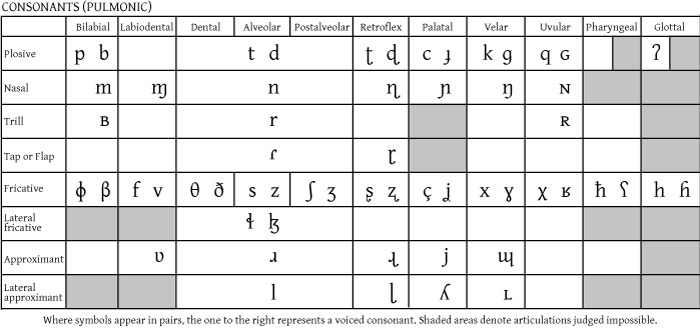
\includegraphics[width=\textwidth]{figures/ipa_consonants_wikimedia.png}


If you remember the periodic table of the elements from chemistry class, you remember that it is organized left to right by the number of electrons in the atom's outermost shell, and  top to bottom by the number of electron shells that orbit its nucleus,  so that column-mates and row-mates share important distinctive properties.  The IPA consonant chart is similarly organized into meaningful rows and columns: from top to bottom by how much the air expelled by the lungs does or does not stop in the mouth in creating that sound, and from left to right by the position in the mouth, from front to back, where the airflow is constricted.

\begin{table}[b]
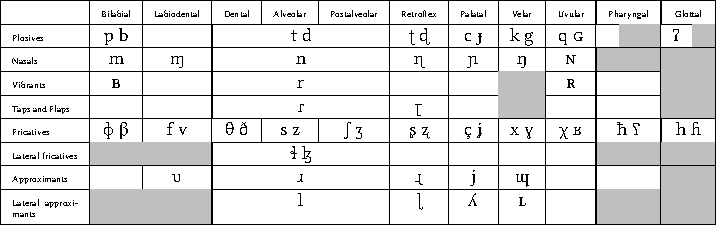
\includegraphics[width=\textwidth]{figures/ipa-table-unicode.pdf}
\caption{IPA consonants}
\label{fig:ipa-consonants}
\end{table}


As seen in Figure~\ref{fig:ipa-consonants}, the top left of the IPA consonant chart represents the sounds [p] and [b] (which basically correspond to their pronunciations in the Latin alphabet), where the air stops fully at the very front of the mouth on the lips.  Moving across, the \keyword{place of articulation} moves further back in the mouth (e.g., [k] and [{g}] are formed by raising the back of the tongue); moving down, the \keyword{manner of articulation} involves less and less stoppage of air, with sounds like [f] and [v] allowing air to flow out of the mouth without stopping.  The sounds [p] and [b] both share the same place (bilabial, involving both lips) and manner (fully stopping the air) of articulation, differing only in \keyword{voicing}: whether the vocal cords are vibrating during the articulation of the sound.  Whenever two sounds share the same cell in the IPA consonant chart, the first one is unvoiced and the second is voiced.



The IPA is designed to represent sounds from any human language, and each individual language uses only a subset of the available possible sounds.  So some of the IPA sounds are not used in English at all, for example the velar fricative [x] used in the German word for `book,' \exword{Buch}. (This [x] is distinct from the orthographic letter \exword{x} of the Latin alphabet, used in \exword{tax} and \exword{exit}: in the IPA, the sound represented by the orthographic \exword{x} in \exword{tax} is [ks], and in \exword{exit} can be either [ks] or [{g}z]!  Which version do you use?).

Turning to the vowels, the IPA vowel chart in Figure~\ref{fig:ipa-vowels} is organized to look like the shape of the mouth, because vowels are distinguished by the place of the tongue in the mouth when the air is expelled.  The top left of the vowel chart is the high, front vowel [i], as in the word \exword{b\uline{ee}} -- here, the tongue is raised and the air is sent through the upper portion of the mouth.  The other sound at the top left of the chart is [y], which is high and front like [i] but also involves \keyword{rounding} of the lips.  This sound is not used in English; English only allows back vowels (created at the back of the mouth, like the vowel [u] in \exword{b\uline{oo}t}), to be rounded.  The front rounded vowel [y] is used in French words such as \exword{t\uline{u}} `you'.

\begin{figure}
% 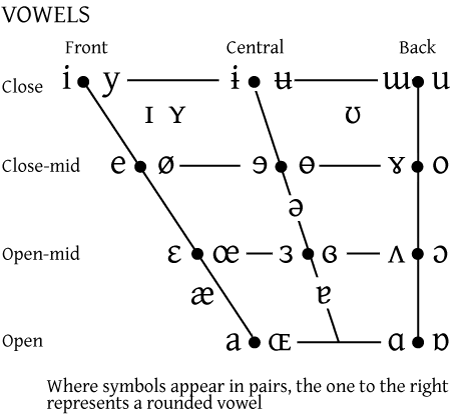
\includegraphics[width=0.7\textwidth]{figures/ipa_vowels_wikimedia.png}
\begin{vowel}
\putcvowel[l]{i}{1}
\putcvowel[r]{y}{1}
\putcvowel[l]{e}{2}
\putcvowel[r]{\o}{2}
\putcvowel[l]{\textepsilon}{3}
\putcvowel[r]{\oe}{3}
\putcvowel[l]{a}{4}
\putcvowel[r]{\textscoelig}{4}
\putcvowel[l]{\textscripta}{5}
\putcvowel[r]{\textturnscripta}{5}
\putcvowel[l]{\textturnv}{6}
\putcvowel[r]{\textopeno}{6}
\putcvowel[l]{\textramshorns}{7}
\putcvowel[r]{o}{7}
\putcvowel[l]{\textturnm}{8}
\putcvowel[r]{u}{8}
\putcvowel[l]{\textbari}{9}
\putcvowel[r]{\textbaru}{9}
\putcvowel[l]{\textreve}{10}
\putcvowel[r]{\textbaro}{10}
\putcvowel{\textschwa}{11}
\putcvowel[l]{\textrevepsilon}{12}
\putcvowel[r]{\textcloserevepsilon}{12}
\putcvowel{\textsci\ \textscy}{13}
\putcvowel{ʊ}{14}
\putcvowel{\textturna}{15}
\putcvowel{æ}{16}
\end{vowel}
\caption{IPA vowels.}
% \caption{IPA vowels (\url{https://commons.wikimedia.org/wiki/File:Ipa-chart-vowels.png})}
\label{fig:ipa-vowels}
\end{figure}

The IPA coheres perfectly to the idea (roughly true in all alphabetic systems) that each symbol represents exactly one sound.  It has the advantage of being unambiguous: A given symbol is pronounced in the same way in all contexts.  And yet, despite these major advantages, the IPA is used mainly by linguists to discuss specific sounds; no one actually uses it as a widespread writing system for disseminating text in any language.  We will explore why not in \chapref{ch:writers-aids}.

%The International Phonetic Alphabet is designed so that each speech sound (from any language) has its own symbol.  This eliminates the need for multiple symbols being used to represent simple sounds and one symbol being used for multiple sounds.  The problem for English is that the Latin alphabet, as we use it, only has 26 letters, but English has more sounds than that.  So, it is no surprise that we find multiple letters like \exword{th} or \exword{sh} being used for individual sounds.

Returning to writing systems used in the real world, the broad class of alphabetic systems also includes \keywordAs{abjads}{abjad} (consonant alphabets), which represent 
consonants only.  Some prime examples are Arabic, Aramaic, and Hebrew.
In abjads, vowels are typically deduced from context or marked by diacritics,  
%The situation with abjads often is a bit more complicated than what we just described, in that characters sometimes represent selected vowels, and often vowel diacritics are available.   
as illustrated by the Hebrew word for \exsent{computer} shown on the
left-hand side of Figure~\ref{fig:hebrew}.

\begin{figure}[htb!]
\mbox{}
\hfill\hfill  \begin{tabular}{l}
      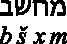
\includegraphics[scale=1.2]{figures/hebrew-computer}\\
      {[maxʃev]}\\[2pt]
      `computer'\\
    \end{tabular}
\hfill
\begin{tabular}{l}
      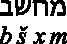
\includegraphics[scale=1.2]{figures/hebrew-computer}\\
      {[mexuʃav]}\\[2pt]
      `is digitized'\\
    \end{tabular}
\hfill
\begin{tabular}{l}
      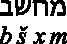
\includegraphics[scale=1.2]{figures/hebrew-computer}\\
      {[mexaʃav]}\\[2pt]
      `with + he thought'\\
    \end{tabular}
\hfill
\hfill
\mbox{}
\caption{Example of Hebrew (abjad) text.}
\label{fig:hebrew}
\end{figure}

The Hebrew word in its character-by-character transliteration
\textit{b\v{s}xm} (read right to left) contains no vowels, so the reader must rely on outside knowledge to supply the
{[a]} and {[e]} vowels shown in the IPA rendering of
the word {[maxʃev]}.  (Hebrew is written
right to left, so the rightmost \textit{m} in the letter-by-letter transliteration corresponds to the 
the first sound that is pronounced, matching the leftmost symbol in the  IPA.  We wrote the letter-by-letter transliteration from right to left to align with the Hebrew letters above.)  As shown in the middle
and righthand side of Figure~\ref{fig:hebrew}, the same string is also compatible with 
 other pronunciations and meanings: Only the consonants are written, so the vowels have to be supplied by the reader's wider knowledge of the language and the context.
	



\subsection{Syllabic systems}

\keywordAs{Syllabic systems}{syllabic system} are like alphabetic
systems in that they involve a mapping between characters and sounds,
but the units of sound are larger, comprising
\keywordAs{syllables}{syllable} made from multiple articulatory gestures.  

All human languages have syllables as basic
building blocks of speech, but the rules for forming syllables differ
from language to language.
For example, in Mandarin Chinese, a syllable consists of a single vowel or diphthong (two vowels within the same syllable), optionally preceded by at most one consonant or affricate (two consonants articulated as one), and optionally followed by a nasal ({[n]} or [ŋ]) or a rhotic sound [ɹ].  Syllables are also distinguished by tone, the contour of pitch throughout the duration of the syllable.  This system gives rise to words, transliterated into the Latin alphabet using the Pinyin system, with tones rendered as diacritics above vowels, such as \exword{t\'ush\={u}gu\v{a}n} `library', \exword{M\v{e}igu\'o} `America', and \exword{x\={i}ngq\'iw\v{u}}  `Friday' (note that \exword{sh} and \exword{ng} each represent single phonetic consonants, [ʃ] and [ŋ], even though these are spelled with two orthographic consonants in the Latin alphabet).

Most of the world's
languages have relatively simple syllables, like Mandarin. This means
that the total number of possible syllables in the language is quite
small, and that syllabic writing systems work well. In English, Russian, and other languages, however, the beginning or end of the syllable may also include a
so-called \keyword{consonant cluster}, such as [sp] and [ɹk] in \exword{\uline{sp}a\uline{rk}}).  This greatly expands the number of
possible syllables.  You could design a syllabic writing system for
English, but it would be unwieldy and difficult to learn, because
there are so many different possible syllables.

There are two main variants of syllabic systems, the first being
\keywordAs{abugidas}{abugida}, or \keywordAs{alphasyllabaries}{alphasyllabary}. 
In these writing systems, the symbols are organized into families.
All the members of a family represent the same consonant, but
they correspond to different vowels. The members of a family also look
similar, but have extra components that are added in order to represent
the different vowels. The distinctive thing about an abugida is that 
this process is systematic, with more or less the same vowel components
being used in each family.

To write a syllable consisting of a consonant and a vowel,
you go to the family for the relevant consonant, then select the
family member corresponding to the vowel that you want. This works 
best for languages in which almost all syllables consist of exactly one
consonant and exactly one vowel.  Of course, since writing is a powerful 
technology, this has not stopped abugidas from being used, with modifications,
to represent languages that do not fall into this pattern. 
One of the earliest abugidas was the Brahmic script, which was in wide use
in the third century BCE, and which forms the basis of many writing systems used
on the Indian subcontinent.

As an example, let us look at the writing system for Burmese, a Sino-Tibetan language spoken in Myanmar.  
%
In
Figure~\ref{fig:burmese-c}, we see a table displaying the base syllables.  Just as in the periodic table of the elements and the IPA of consonants, the rows and columns are meaningful: The top row corresponds to various consonants made by raising the back of the tongue to the velum (soft palate); the leftmost column corresponds largely to voiceless consonants, formed without vibration of the vocal cords.

\begin{figure}
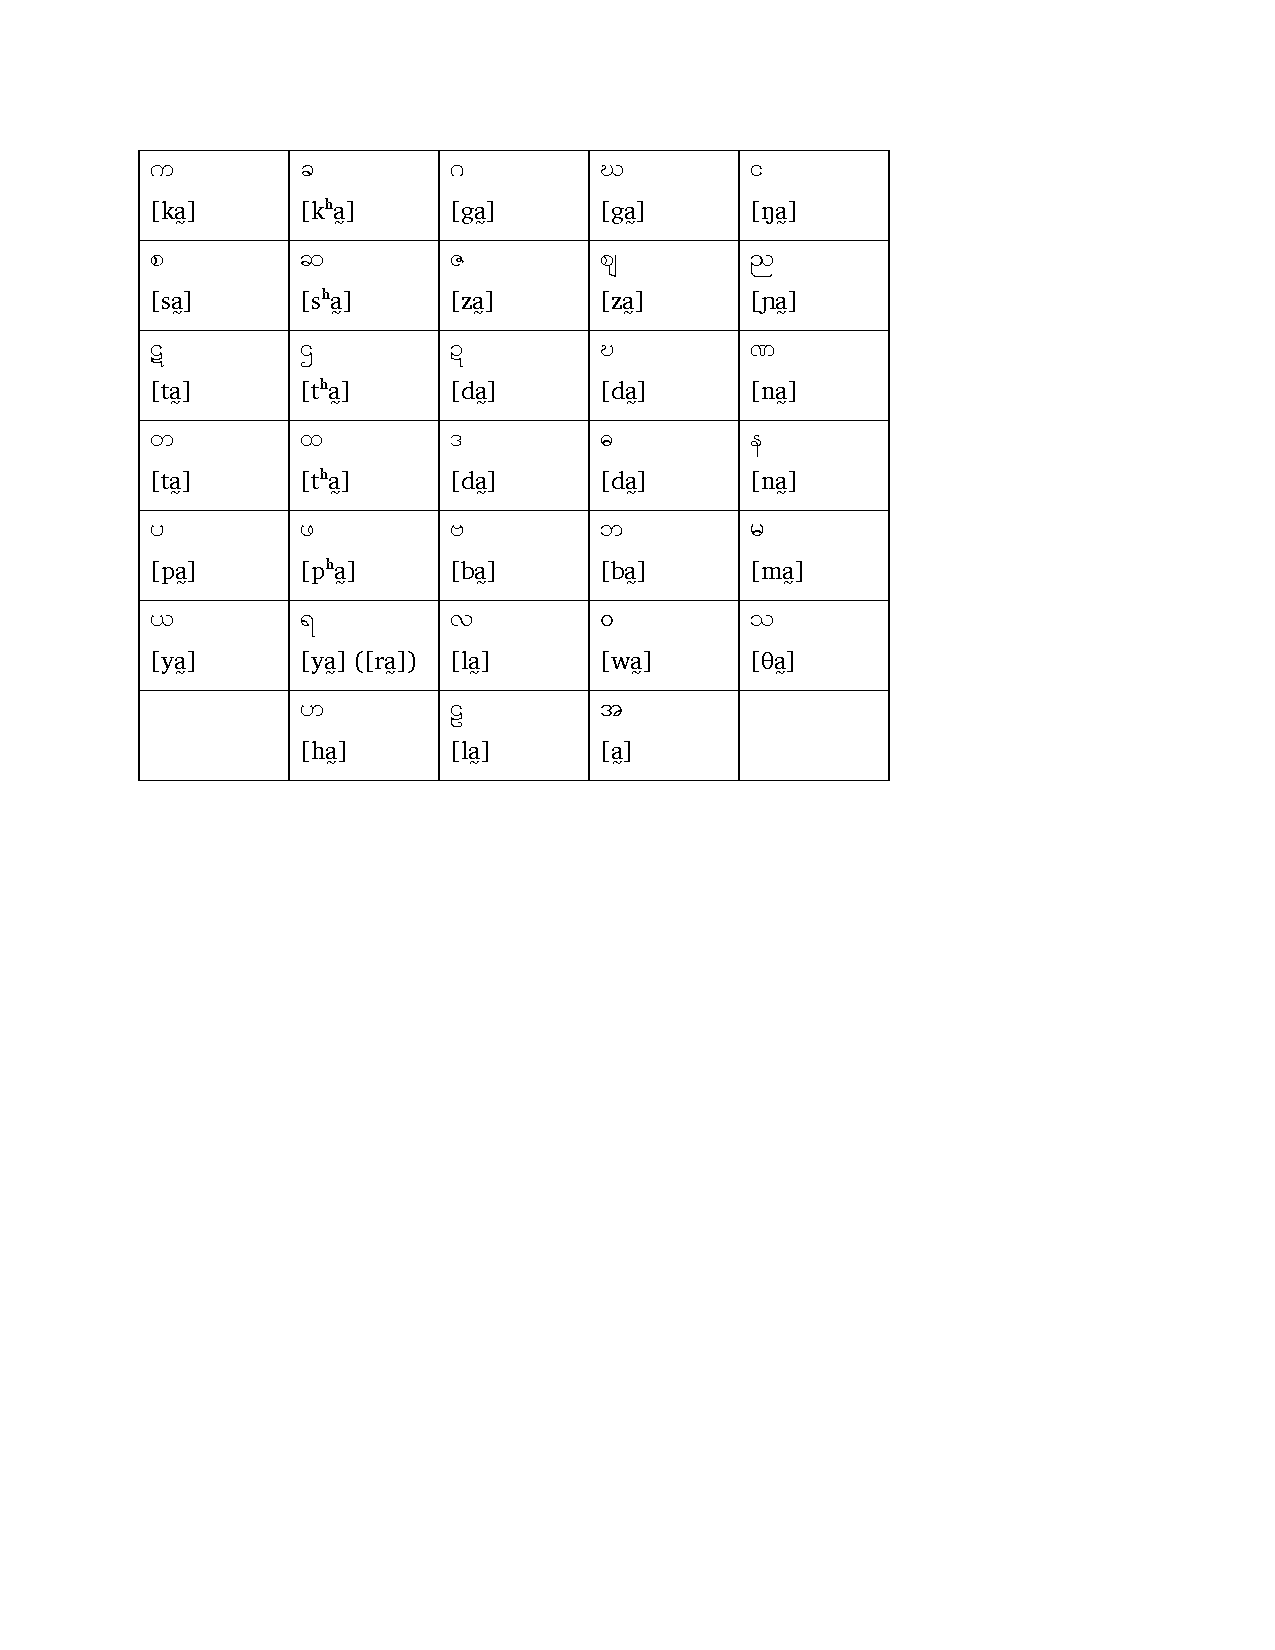
\includegraphics[scale=.7,clip,trim=65 416 184 70]{figures/burmese-consonants}
\caption{Base syllables of the Burmese abugida.}
\label{fig:burmese-c}
\end{figure}

As you can see in the table, every syllable has a default vowel of
{[\~ɐ]}.  This default vowel can be changed by adding
diacritics, as shown in Figure~\ref{fig:burmese-v}, for syllables
which start with {[k]}.

\begin{figure}
  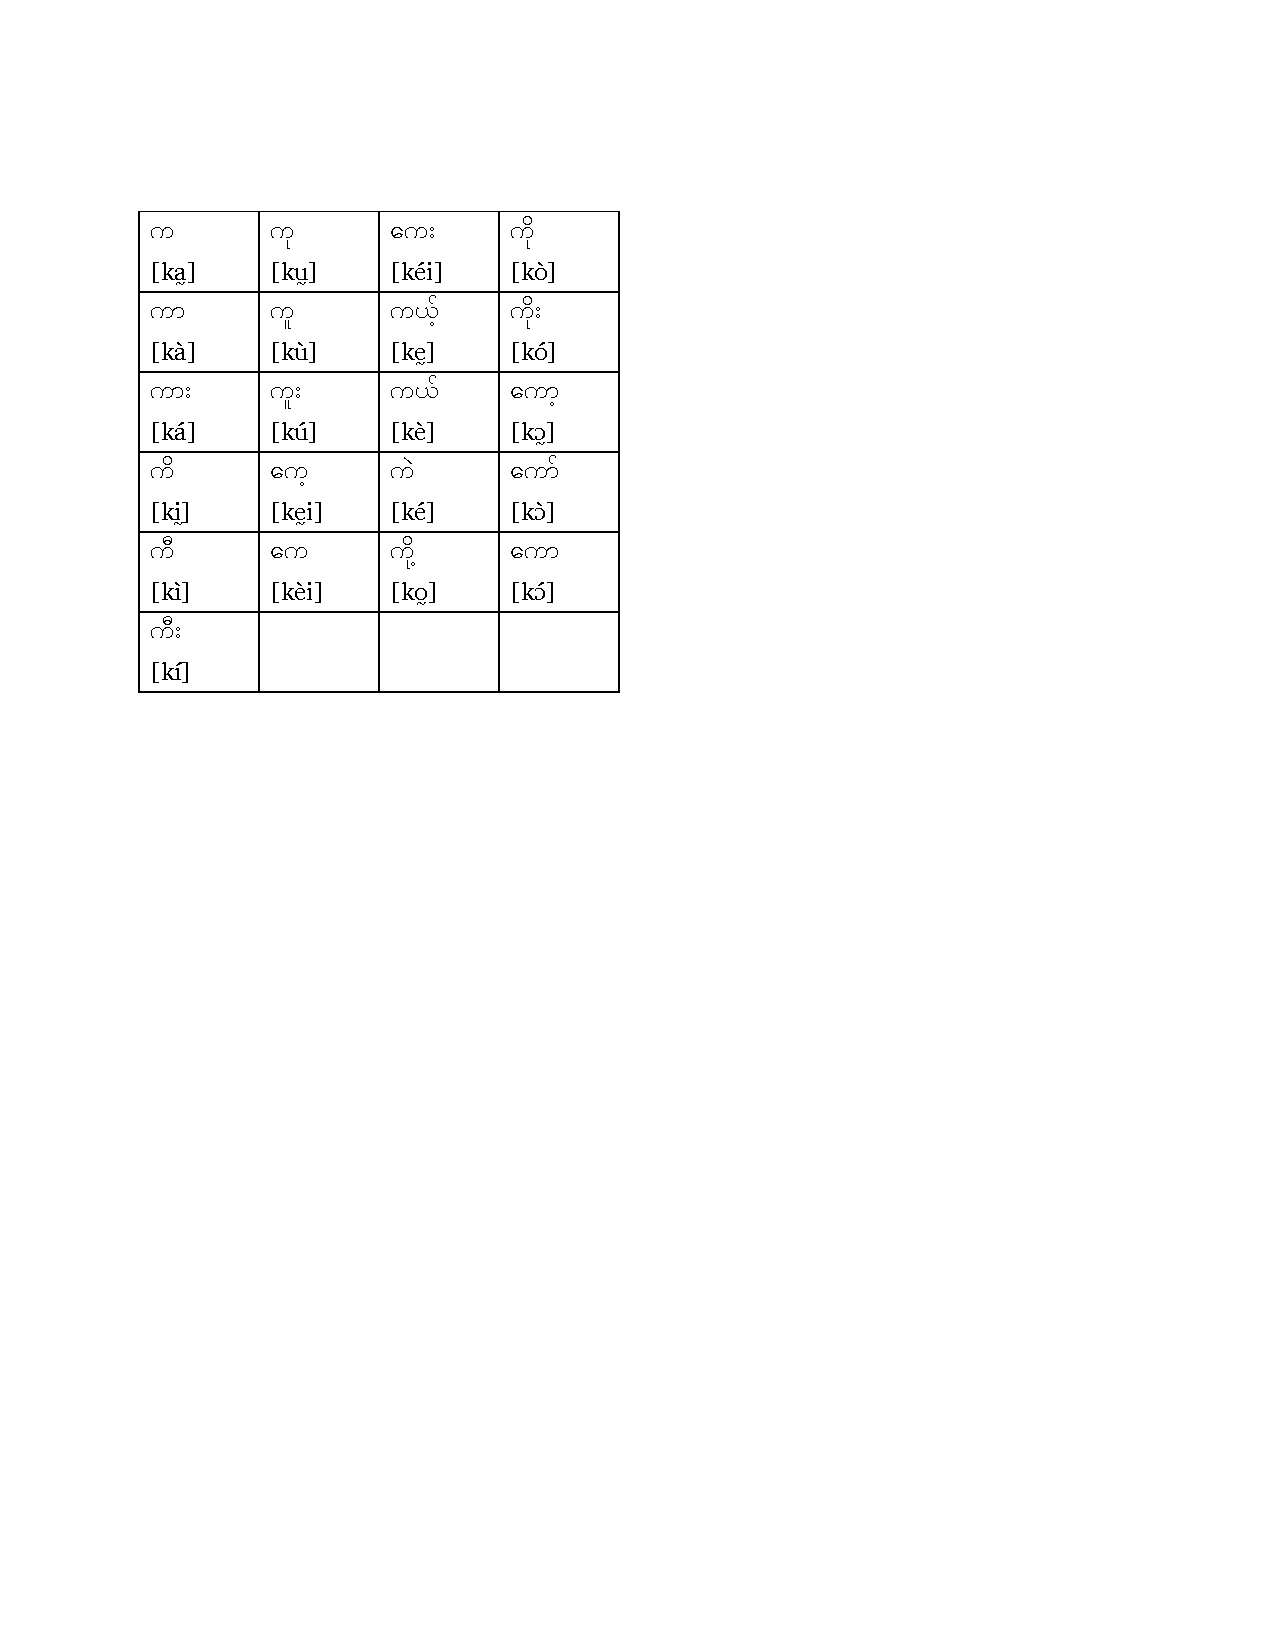
\includegraphics[scale=.7,clip,trim=65 455 314 100]{figures/burmese-vowels}
\caption{Vowel diacritics of the Burmese abugida.}
\label{fig:burmese-v}
\end{figure}

We can see that the base character remains the same in all cases,
while diacritics indicate the vowel change.  Even though there is some
regularity, the combination of the base character plus a diacritic
results in a single character, which distinguishes abugidas from the
alphabets in Section~\ref{sec:alpha}. In this case, characters are written from
left to right, but the diacritics appear on any side of the
base character.  

The second kind of syllabic system is the \keyword{syllabary}.  These
systems use distinct symbols for each syllable of a language.
An example syllabary for Vai, a Niger-Congo language spoken in
Liberia, is given in Figure~\ref{fig:vai}.

\begin{figure}[H]
  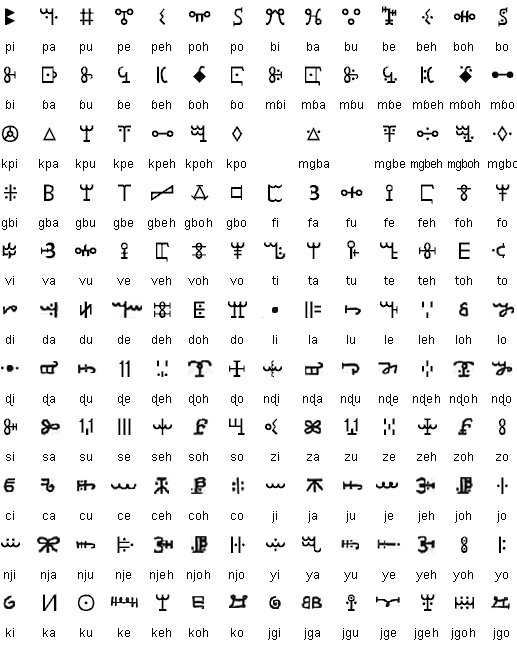
\includegraphics[width=0.7\textwidth]{figures/vai}
  \caption{The Vai syllabary (\url{https://commons.wikimedia.org/wiki/File:Vai.gif}, uploaded by user Neal; public domain information with no claim to original authorship).}
\label{fig:vai}
\end{figure}

Whereas the syllables in an abugida are organized into some sort of pattern, the syllables of a general syllabary need not be.  For example, in Vai, 
it is hard to see a connection between the symbols for {[pi]}
and {[pa]} even though they begin with the same consonant, or any connection between the symbols
for {[pi]} and {[di]} even though they end with the same vowel.

\subsection{Logographic writing systems}
\label{sec:logographic-writing-systems}

The final kind of writing system to examine involves
\keywordAs{logographs}{logograph}, or logograms.  A logograph is a symbol which
represents a unit of meaning, as opposed to a unit of sound.  Among writing systems for natural languages, some (such as Chinese) use logographic elements, but cannot be considered purely logographic because they include phonetic information as well.
  

A purely logographic system is exemplified by the symbols used on
signs at United States National Parks shown in Figure~\ref{fig:usnps}.  These
are referred to as \keywordAs{pic\-to\-graphs}{pictograph}, or
pictograms, because they essentially are pictures of the items they
refer to.  The upper left symbol, for instance, refers to camping by
means of displaying a tent.

\begin{figure}
    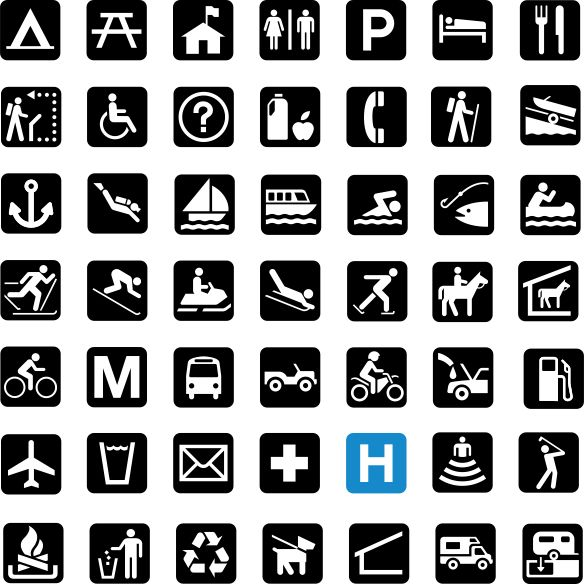
\includegraphics[width=.7\textwidth]{figures/usnps}
    \caption{U.S. National Park Service pictographic symbols (\url{https://commons.wikimedia.org/wiki/File:National_Park_Service_sample_pictographs.svg}, uploaded by user Tkgd2007; public domain as the work of the United States government).}
    \label{fig:usnps}
\end{figure}

Some modern written characters evolved from a more pictographic representation
into a more abstract symbol.  For example, we can look at the development of the Chinese character for
`horse', pronounced (in the Pinyin romanization) as \exword{m\v{a}}, as in Figure~\ref{fig:horse}. 
Originally, the character very much resembled a horse, but after
evolving over the centuries, the modern character only bears a
faint resemblance to anything horse-like.

\begin{figure}
    \begin{tabular}{cccccc}
      
\includegraphics[width=.1\textwidth]{figures/01-chinese-oracle} &
      
\includegraphics[width=.1\textwidth]{figures/02-chinese-bronze} &
      
\includegraphics[width=.1\textwidth]{figures/03-chinese-bigseal} &
      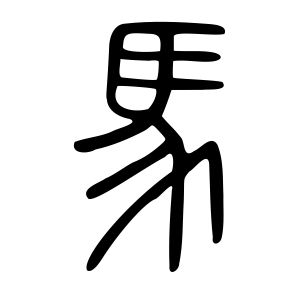
\includegraphics[width=.1\textwidth]{figures/04-chinese-seal} &
      
\includegraphics[width=.1\textwidth]{figures/05-chinese-kaishu-trad} &
      
\includegraphics[width=.1\textwidth]{figures/06-chinese-simplified.jpg} \\
      Oracle & Bronze & Big Seal & Small Seal & Traditional & Simplified\\ 
      script & script & script   & script     & script    & script   \\ 
    \end{tabular}
    \caption{Evolution of the Chinese character for `horse'. (\url{https://commons.wikimedia.org/wiki/Commons:Ancient_Chinese_characters_project}, public domain because ancient scripts predate the concept of copyright).}
    \label{fig:horse}
\end{figure}

  
Not only has the logogram for \exword{horse} become less horse-like over time, but it is also used to encode the sound \exword{m\v{a}} rather than the meaning ``horse'' in \keywordAs{semantic-phonetic compounds}{semantic-phonetic compound} such as the character for `mother', pronounced \exword{m\={a}}.  The Chinese words for `horse' and `mother' are pronounced the same except for their tone, the pitch contour which distinguishes words in some languages: \exword{M\v{a}} `horse' uses a down-up tone, while \exword{m\={a}} `mother' uses a high flat tone.  In writing, the character for \exword{m\={a}} `mother' has a semantic element on the left, the character for \exword{woman} (phonetically silent here, but pronounced \exword{n\"u} on its own), and a phonetic element on the right: The character for `horse', pronounced \exword{m\v{a}}.  The semantic-phonetic compound represents that \exword{m\={a}} `mother' is semantically woman-like and phonetically horse-like.  Both  pieces of information are useful, but a Chinese reader still has to memorize the specific sound-meaning correspondence evoked vaguely by these clues.


%There are characters in Chinese which prevent us from calling the writing system a fully meaning-based system. \keywordAs{Semantic-phonetic compounds}{semantic-phonetic compound} are symbols with a meaning element and a phonetic element.  An example is given in Figure~\ref{fig:s-p-compounds}, where we can see that, although both words are pronounced the same, they have different meanings depending upon the semantic component.  Of course, it is not a simple matter of adding the phonetic and semantic components: knowing that the meaning component of a semantic-phonetic compound is `wood' by itself does not tell you that the meaning of the compound is \exsent{timber}.

\begin{figure}
% 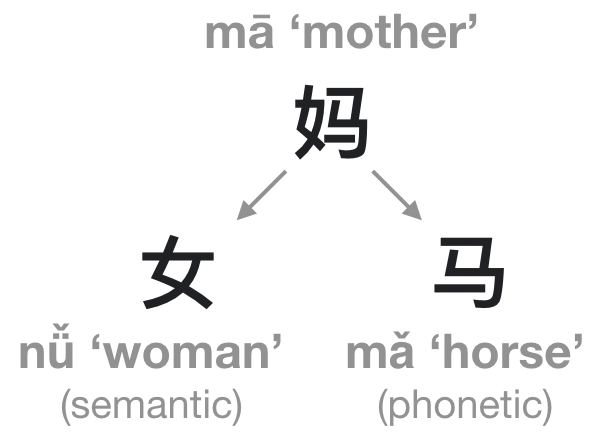
\includegraphics[width=.4\textwidth]{figures/chinese-compound-ma.jpg}
\begin{forest}for tree={align=center,edge={->}}
[{m\=a\\{\cn 妈}}
	[{{\cn 女} \\n\v{ü} `woman' \\ {\footnotesize (semantic)}}]
	[{{\cn 马}\\m\v{a} `horse' \\ {\footnotesize (phonetic)}}]
]
\end{forest}

\caption{Semantic-phonetic compound character \exword{m\={a}} `mother' in the Chinese writing system.}
\label{fig:s-p-compounds}
\end{figure}
% I redid this based on my own knowledge of Chinese. I thought it was better to keep talking about MA/horse than to introduce the new example of CAI/valuables/wood.

More broadly, Chinese semantic-phonetic compounds illustrate that the Chinese writing system is not purely logographic; the phonetic portion of the compound still provides information about pronunciation to complement the logographic representation of meaning.


\subsection{More hybrid systems}

You can already see from the Chinese writing system (a blend of syllabic and logographic elements) that the boundaries between alphabetic, syllabic, and logographic writing systems can be blurred.  Many systems use a hybrid of these elements.


The writing system for Korean uses both
alphabetic and syllabic concepts.  This writing system is referred to as \emph{Hangul} (or \emph{Hangeul}) and was developed in
1444 during the reign of King Sejong.  The Hangul system contains 24
letter characters, fourteen consonants and ten vowels.  These alphabetic elements are grouped into syllabic units.
%
We can see an example in Figure~\ref{fig:hangul}, which
shows how individual alphabetic characters together form the syllabic
characters for \exword{han} and \exword{geul}.

\begin{figure}
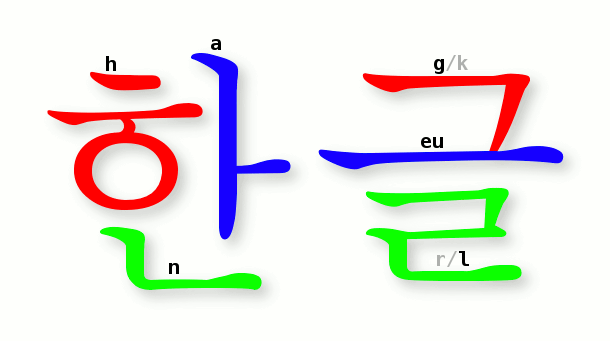
\includegraphics[width=.8\textwidth]{figures/Hangeul}
\caption{Composition of the characters for \exword{Hangeul} (\url{https://commons.wikimedia.org/wiki/File:Hangeul.png}, uploaded by user IGEL with CC share-alike license).}
\label{fig:hangul}
\end{figure}

Within a syllable block, the alphabetic elements are organized mostly vertically; but the syllables are written left to right. In South Korea, \emph{hanja}
(logographic Chinese characters) were historically used too, for a blend of all three (alphabetic, syllabic, and logographic) elements.
      

Braille is a writing system for people with vision impairments which makes it possible to read through touch.  We
can see the basic alphabet in Figure~\ref{fig:braille}.

\begin{figure}
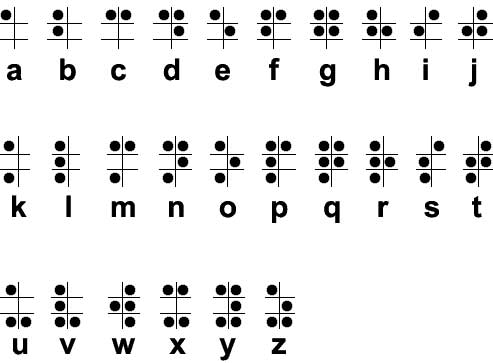
\includegraphics[width=.6\textwidth]{figures/braille-alphabet}
\caption{The Braille alphabet (\url{https://commons.wikimedia.org/wiki/File:Braille_alfabet.jpg},  uploaded by user Maikel Honcoop; public domain information with
no claim to original authorship).}
\label{fig:braille}
\end{figure}

The Braille system works by using patterns of raised dots arranged in
cells of up to six dots, in a three-by-two configuration.  Each pattern
represents a character, but some frequent words and letter
combinations have their own pattern.  For instance, the pattern for
\exword{f} also indicates the number \exword{6} (because it is the sixth letter of the alphabet) and the word \exsent{from} (which starts with \exword{f}) -- to be disambiguated by the context.
So, even though it is at core an alphabet, it has some logographic
properties.

 
As one of the world's oldest writing systems, Ancient Egyptian hieroglyphics seem to record a brainstorming session in all the different ways that language  can be recorded in text.   At different times, Ancient Egyptians tried writing right to left, left to right, and top to bottom.  Some Ancient Egyptian glyphs represented a single sound, as in an alphabetic system; but vowels were usually not represented, as in an abjad.   Others represented two or three consonants at once, similar to a syllabic system in that one character reflects multiple sounds.  Still others represented a meaning, as in a logographic system; some of these were pronounced as words, but other ``mute'' logograms/pictograms were meant to clarify the meaning of the text without being pronounced (a pictogram of a boat might be added to clarify the meaning of the alphabetic spelling of the word for \exword{boat}).   These ancient pictograms share striking similarities to the non-pronounced \keyword{emoji} (see the Under the Hood box) that have become increasingly popular in recent years to enrich the socio-emotional meaning of text.

\begin{tblsfilledsymbol}{\underthehoodsubsection{Emoji}}{glass}
\begin{underthehood}

After this discussion of writing systems, you might be wondering about the status of  modern digital symbolic systems, such as \keyword{emoji}.  Emoji appear logographic, in that they depict meaning: A smiley face depicts a cheerful demeanor.

So do emoji constitute a logographic writing system?  No, because they are not a writing system!  Recall that a writing system is ``a system of more or less permanent marks used to represent  an  utterance  in  such  a  way  that  it  can  be  recovered  more  or less  exactly  without  the  intervention  of  the  utterer'' \citep{daniels:bright:96} -- by representing some portion(s) of the sound/meaning pairings of a particular language.  Emoji do not represent utterances or sound/meaning pairings in any particular language.  Instead, many emoji (at least the most common ones, such as the laughing-crying face \laughing \text{} and the heart-eyes face \heart) represent the unpronounceable, non-verbalized emotions (conveyed in real life by facial expressions, gestures, and voice quality), which are otherwise absent from writing.




Emoji have historical antecedents in emoticons, such as the smiley face rendered by punctuation :-), and web abbreviations for non-speech communicative acts, such as \exword{LOL}.  Emoji were added to some Japanese phones in 1999  by the designer Shigetaka Kurita, and became part of Unicode in 2010 (see Section~\ref{sec:bytes} for more on Unicode).  To this day, the Unicode Consortium manages the set of emoji, vets petitions for new emoji, and records statistics about the most popular ones.



 Like traffic-sign pictograms, emoji are relatively universal: Whether you speak English or German, you know the meaning of the heart-eyes emoji \heart.  In contrast, written representations of actual languages are not universal; if you only speak English, you will not know the meaning of the German (written) word \exword{L\"acheln} `smile'. Emoji can be universal specifically because they do not represent utterances in any particular language.
 
Illustrating the limited expressive power of emoji, \emph{Emoji Dick} \citep{Benenson:2010} gathers English-to-emoji  ``translations'' (written by workers on the Amazon Mechanical Turk gig platform, commissioned by the entrepreneur Fred Benenson) of sentences from the classic novel \emph{Moby Dick} by Herman Melville.  Imagine trying to read \REF{emojib} without the corresponding English sentence!  Since emoji do not constitute a writing system for a language, much of the English sentence's information is lost: There is no first-person pronoun and no way of representing the name \exword{Ishmael} in emoji.  Instead, the ``emoji sentence'' \REF{emojib} includes information about a boat and a whale,  not present in the English original. 

 \ea \ea  Call me Ishmael.
    \ex \label{emojib} \telephone \beardman \sailboat \whale \okayhand 
\z
\z


In sum, emoji carry important communicative meaning and can be used to represent emotions, non-speech gestures, and some concrete entities such as boats and whales -- but they do not constitute a fully expressive writing system for a human language.


\end{underthehood}
\end{tblsfilledsymbol}



\begin{tblsfilledsymbol}{\underthehoodsubsection{Online gig platforms}}{glass}
 \begin{underthehood}

We just saw that the 2010 book \emph{Emoji Dick} was created by paying gig workers on Amazon's Mechanical Turk platform to ``translate'' English sentences from the novel into emoji.    Mechanical Turk takes its name from a toy created in the 1770s for the Austrian court, a doll dressed in  stereotypical Turkish clothing, which was represented as a chess-playing robot but actually concealed a human inside who moved the pieces.  The Mechanical Turk doll looked like artificial intelligence, but contained a human at its core.  Similarly, Amazon's platform is meant to operate as easily as an automated system -- you can post a task online and download your results in just a few hours -- but leverages the human intelligence of gig workers.  Mechanical Turk is one of several such platforms, including Prolific and CrowdFlower, which are widely used in language research and technology.

\newpage
In psychology and linguistics research, it is common to conduct text-based experiments.  For example, \citet{Loftus:1975} played a video of a car driving on a road, and then asked some people, \exsent{How fast was the car going on the country road?} while asking others, \exsent{How fast was the car going when it passed the barn?}.   Later, both groups were asked if they saw a barn.  In fact, the video did not show a barn -- but the people who had read the sentence mentioning a barn were far more likely to mis-remember one!  The study famously shows that the wording of a question can be used to implant a false memory.  Although the study was originally run in-person with university students as participants, it serves as an example of a study that could be run online -- far more quickly and cheaply.  To recruit two hundred university students to come to a physical laboratory to do a pen-and-paper experiment would take thousands of dollars and weeks; to recruit the same number of people to do a study on their own device from home would take a few hundred dollars and an afternoon.

Such web surveys can serve all sorts of purposes.  A business might ask people whether they've heard of their product or how much they like it; a political campaign might ask what people think of a candidate or a message.  In language technology, one might recruit people to write captions for images (free text), flag comments as hateful or not (labels from a closed class), or provide a rating for the politeness of a request (a continuous scale).  These data can provide insight on their own, but can further be used as input for a system that ``learns'' to handle new data in the same way -- for example, learning to label new comments as hateful or not, generalizing the labels provided by humans.  Such machine learning tools are discussed further in \chapref{ch:text-classification}.

When gathering such data on the web, researchers worry about quality: Are the workers actual humans, or are they bots?  If they are humans, are they paying attention or clicking mindlessly through the task?  A researcher might add questions to their study specifically to  flag poor-quality respondents, but spammers may also find ways around these questions, creating an arms race.  Moreover, who are these humans?  Is this sample biased in a way that might limit the generalizations that can be drawn from their data?

Gig platforms also raise questions about ethics: Are workers being fairly compensated for their labor?  Are they earning minimum wage (in what location?) -- hard to count when they may do ten different short tasks in an hour?  How many hours do they work on a gig platform, and should they earn overtime or benefits?  How should they be credited intellectually for their output or the technologies built from it?

Over time, spammers get more sophisticated and gig-work regulations evolve, so the future of such platforms remains in flux; but they are likely to remain a crucial tool in language technology.

\end{underthehood}
\end{tblsfilledsymbol}






\section{Digital writing}
\label{sec:encoding-written-language}

We have explored how language pairs sounds/signs with meaning, and how writing systems encode some portion of that pairing (sound and/or meaning).  Next, we explore how writing systems are in turn encoded digitally, allowing computers to process text.

Before exploring how computers can encode diverse writing systems, we begin with a more basic question:  How do computers encode anything?

\subsection{Bits and bytes}

To answer that, we need to know that information on a computer is
stored in \keywordAs{bits}{bit}.  We can think of the memory of a computer
as, at its core, a large number of on-off switches.  A bit has two
possible values, 1 (yes) or 0 (no), allowing us to flip the switches
on or off.  A single bit on its own does not convey much information,
but multiple bits can come together to make meaningful patterns.  It
is thus often more convenient to speak of a \keyword{byte}, or a
sequence of 8 bits, e.g., 01001010.

These sequences of bits tell the computer which switches are on and
which are off, and -- in the context of writing systems -- a particular
character will have a unique pattern of on-off switches.  Before we
fully spell that out, though, let us consider a better way to think of
sequences of bits, other than just a sequence of mindless 0s and 1s.

Bit sequences are useful because they can represent numbers, in
so-called \keyword{binary} notation.  They are called binary because
there are only two digits to work with.  The base ten numbers we
normally use have columns for ones, tens, hundreds, etc.; likewise,
binary numbers have their own columns, for ones, twos, fours, eights,
etc.  In addition to base two and base ten, you can find encodings
such as \keyword{hexadecimal}, where there are 16 digits (0-9 and then
the letters A-F).

In \keyword{Big Endian} notation, the most significant bit is the
leftmost one; this is the standard way of encoding and is parallel to
decimal (base ten) numbers.  The positions in a byte thus encode the
top row of Table~\ref{fig:big-endian}.  As we can see in the second
row, the positions for 64, 8, and 2 are ``on,'' and
64+8+2 equals 74. The binary (base two) number 01001010 therefore
corresponds to the decimal number 74.

\begin{table}
\begin{tabular}{rrrrrrrrrr}
\lsptoprule
128 & 64 & 32 & 16 & 8 & 4 & 2 & 1 \\
\midrule
0 &  1 &  0 &  0 & 1 & 0 & 1 & 0 \\
\lspbottomrule
\end{tabular}
\caption{The number 74 in Big Endian notation.}
\label{fig:big-endian}
\end{table}
        

%\mparshift{\baselineskip}
\keyword{Little Endian} notation is just the opposite, where the most
significant bit is the rightmost one, but it is less common.
In both cases, the columns are all multiples of two.  This is just
like with decimal numbers, where the columns are all multiples of ten.
As each digit is here limited to either 0 or 1 (two choices), we have
to use multiples of two.

\subsection{Converting decimal numbers to binary}

Although many of you are likely already familiar with binary numbers,
it is instructive to see how to convert from decimal to
binary notation.  
We will consider the division method of conversion and walk through an
example, converting the decimal number 9 into a 4-bit binary number.

The division method is easy to calculate and moves from the least significant 
to the most significant bit.  Because every column has a value which is a multiple of
two, we divide by 2 with every step.  In
Table~\ref{fig:bit-division}, for example, we divide 9 by 2 and find
that we have a remainder.  A remainder after dividing by 2 means that
we started with an odd number.  Since 9 is odd, the rightmost bit
should be 1.

\begin{table}
\begin{tabular}{llr}
\lsptoprule
Decimal & Remainder? & Binary\\
\midrule
9/2 = 4 & yes & \textbf{1}\\
4/2 = 2 & no & \textbf{0}1\\
2/2 = 1 & no & \textbf{0}01\\
1/2 = 0 & yes & \textbf{1}001\\
\lspbottomrule
\end{tabular}
\caption{The division method.}
\label{fig:bit-division}
\end{table}

The trick now is to take the resulting value, in this case 4, and
divide it by 2.  The same principle is at work here: If there is no
remainder, it means that the starting number (4) was even, and this
bit needs to be switched off for that to happen. The remaining calculations work the same way, as shown in Table~\ref{fig:bit-division}.


\subsection{Using bytes to store characters}
\label{sec:bytes}

With 8 bits (a single byte) and each byte storing a separate
character, we can represent 256 different characters ($= 2^{8}$).
This is a sufficient amount for many applications and more than enough
for anyone wishing to simply type in Latin characters for English.
With 256 possible characters, we can store every single letter used in
English, plus all the auxiliary characters such as the comma, the
space, the percent sign, and so on.

\subsubsection{ASCII}

One of the first encodings for storing English text used only 7 bits,
thus allowing for 128 possible characters.  This is the
\keyword{ASCII} encoding, the American Standard Code for Information
Interchange.  Figure~\ref{fig:ascii} shows most of the ASCII chart.

\begin{figure}
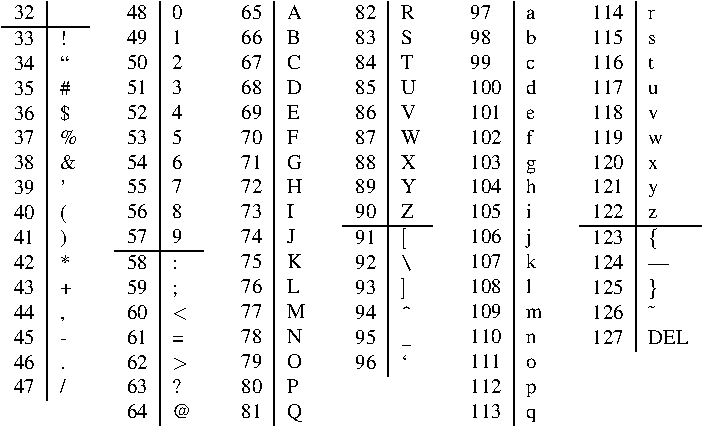
\includegraphics[width=\textwidth]{figures/ascii}
\caption{The ASCII chart.}
\label{fig:ascii}
\end{figure}

Omitted from the chart are codes 1--31 since
these are used for control characters, such as a backspace, line feed,
or tab.  The numeric order reflects alphabetic
ordering (e.g., 65 through 90 for uppercase letters), so it is easy to alphabetize the letters by comparing numbers.  Although we have
written the base ten number, for ease of reading, the binary number is
what is used internally by the computer.

  

You might already be familiar with ASCII or other character encoding
systems, as many communications over email and the internet inform you
as to different encodings.  
Emails come with lots of information about themselves.  Specifically,
Multipurpose Internet Mail Extensions (MIME) provide
\keyword{meta-information} on the text, or information which is part
of the regular message, but tells us something about that message.
MIME information tells us, among other things, what the character set
is; en example can be seen in \REF{mime}.  


\ea \label{mime}  \texttt{Mime-Version: 1.0} \\
   \texttt{Content-Type: text/plain; charset=US-ASCII} \\
   \texttt{Content-Transfer-Encoding: 7bit}
\z 

\subsubsection{Unicode}

As you may recall, one of our goals is to be able to
encode \emph{any} language.  With only 128 possible characters, ASCII
clearly is insufficient for encoding the world's writing systems.
How, then, do we go about encoding writing systems other than the
Latin alphabet?

One approach is to simply extend the ASCII system with various other
systems.  For example, ISO-8859-1 is an 8 bit encoding that in
addition to ASCII includes extra letters needed for French, German,
Spanish, and related languages; ISO-8859-7 is for the Greek alphabet;
ISO-8859-8 for the Hebrew alphabet; and JIS-X-0208 encodes Japanese
characters.  While multiple encoding systems make it possible to
specify only the writing systems one wants to use, there are potential
problems.  First, there is always the potential for misidentification.
Two different encodings can use the same number for two different
characters or, conversely, different numbers for the same character.
If an encoding is not clearly identified and needs to be guessed,
e.g., by a web browser displaying a web page that does not specify the
encoding explicitly, the wrong characters will be displayed.
Secondly, it is a hassle to install and maintain many different
systems in order to deal with various languages.

Unicode\footnote{\url{https://unicode.org}, accessed 2024-05-23.} is a system that addresses
these problems by having a single representation for every character
in any existing writing system. 
While we have some idea about the
variety of writing systems, based on the earlier discussion, we may not have a good feel for how many
characters there are to encode in the world.  Unicode, version 14.0,
has codes for over 144,000
characters from alphabets, syllabaries, and logographic systems.
While this sounds like a lot, it should be noted that Unicode uses 32
bits to encode characters.  The number of distinct characters a system
can encode is equal to $2^n$, where $n$ is the number of bits: With 7
bits, we had $2^7$ (= 128) possibilities.  With 32 bits, we can store
$2^{32} = 4,294,967,296$ unique characters.  

In other words, Unicode allows for
over four billion characters, yet only needs about 150,000.  If we use
32 bits to encode every character, that will take up a lot of space.
It seems like ASCII is better, at least for English, as it only takes
7 bits to encode a character.  Is there any way we can allow for many
characters, while at the same time only encoding what we really need
to encode?

Unicode's solution is to offer three different versions, which
allow for more compact encodings: UTF-32, UTF-16, and UTF-8.  UTF-32
uses 32 bits to directly represent each character, so we will face
more of a space problem with it.  UTF-16, on the other hand, uses 16
bits ($2^{16} = 65,536$), and UTF-8 uses 8 bits ($2^{8} = 256$).

This raises the question: How is it possible to encode $2^{32}$
possibilities in 8 bits, as UTF-8 does?  The answer is that UTF-8 can
use several bytes to represent a single character if it has to, but it
encodes characters with as few bytes as possible by using the highest
(leftmost) bit as a flag.  If the highest bit is 0, then this
is a single character or the final character of a multi-byte
character.  For example, 01000001 is the single-character code for
\exword{A} (i.e., 65).  If the highest bit is 1, then it is part of a
multi-byte character.  In this way, sequences of bytes can
unambiguously denote sequences of Unicode characters.  One nice
consequence of this set-up is that ASCII text is already valid UTF-8.

More details on the encoding mechanism for UTF-8 are given in
Table~\ref{fig:utf8-bytes}.  An important property here is that the
first byte unambiguously tells you how many bytes to expect after it.
If the first byte starts with 11110xxx, for example, we know that with
four 1's, it has a total of four bytes, i.e., there are three more
bytes to expect.  Note also that all non-starting bytes start with 10,
indicating it is \emph{not} the initial byte.

  \begin{table}
    \begin{tabular}{cccccc}
    \lsptoprule
      Byte 1 & Byte 2 & Byte 3 & Byte 4 & Byte 5 & Byte 6 \\\midrule
      0xxxxxxx & \\
      110xxxxx & 10xxxxxx \\
      1110xxxx & 10xxxxxx & 10xxxxxx\\
      11110xxx & 10xxxxxx & 10xxxxxx & 10xxxxxx\\
      111110xx & 10xxxxxx & 10xxxxxx & 10xxxxxx & 10xxxxxx\\
      1111110x & 10xxxxxx & 10xxxxxx & 10xxxxxx & 10xxxxxx & 10xxxxxx\\
    \lspbottomrule
    \end{tabular}
  \caption{UTF-8 encoding scheme.}
  \label{fig:utf8-bytes}
  \end{table}

To take one example, the Greek character $\alpha$ (``alpha'') has a
Unicode code value of 945, which in binary representation is 11
10110001.  With 32 bits, then, it would be represented as: 00000000
00000000 00000011 10110001.  The conversion to UTF-8 works as follows:
if we look at the second row of Table~\ref{fig:utf8-bytes}, we see
that there are 11 slots (represented by the repeated character \exword{x}), and we have 10 binary digits.
The ten-digit number 11 10110001 is the same as the 11-digit 011
10110001, and we can rearrange this as 01110 110001, so what we can do
is insert these numbers into the position held by the \exword{x} characters in the second row:
110\textbf{01110} 10\textbf{110001}.  This is thus the UTF-8
representation.

\section{Spoken language}
\label{sec:encoding-speech}
 
To review, we have explored how language pairs sounds/signs with meaning; how different writing systems encode some portions of that pairing (sound and/or meaning); and how writing systems are in turn encoded on computers in bits and bytes.  Next, we return to the sounds of spoken language and how these too can be encoded digitally, allowing computers to process and produce speech.
  
%We saw above that computers can readily represent and process language in the form of text. While traditionally this has also been the focus of computer-based language analysis, in recent years spoken language interaction is increasingly supported . 
%from digital assistants such as Alexa and Siri spoken language dialogue systems to autom

%Even speech-based dialog systems such as Siri and Google Home map speech to text and back to speech again, using text as the medium for calculating what to say next.  But how do computers map from speech to text and vice versa?\mad{Do we want more on why speech is important in its own right? (Or maybe not, since we focus mainly on text?)}
%\wdm{Some pointers we could add following our application-driven theme are: Alexa, Siri, and ilk, as well as \href{https://youglish.com/}{Youglish}.}

\subsection{The nature of speech}

In order to deal with speech, we have to figure out what it looks
like.  As we saw above in our tour of writing systems, we can \keyword{transcribe} speech into orthographic text or the International Phonetic Alphabet, but first we have to understand the input to such a transcription as a stream of sound.

%It is very easy to visualize spoken language if we think of it as phonetically transcribed into individual characters, but to \keyword{transcribe}, or write down, the speech into a \keyword{phonetic alphabet} (such as the IPA we saw before) is extremely expensive and time-consuming. To better visualize speech and thus encode it on a computer, we need to know more about how speech works and how to measure the various properties of speech.  Then, we can start to talk about how these measurements correspond to sounds we hear.  

We segment speech into words and sounds in our minds and write spaces
between words orthographically, but speech is actually a
\keyword{continuous} and undifferentiated stream of sound. Sounds are
articulated in quick and overlapping succession, so it is hard for a
computer to tell where one sound ends and another begins.
Additionally, people have different accents and different vocal tracts
and thus say things differently.  Two people can say the same word,
and it will come out differently.

Furthermore, the way a particular sound is realized is not consistent
across utterances, even for one person.  What we think of as one sound
is not always said the same.  For example, there is the phenomenon
known as \keyword{coarticulation}, in which neighboring sounds affect
the way a sound is uttered.  
The sound for \exword{k} is said
differently in \exword{\uline{k}ey} and the first sound in \exword{\uline{k}ookaburra}.  (If you do not believe
this, stick one finger in your mouth when you say \exsent{key} and
when you say \exword{koo}; for \exword{key} the tongue touches the finger, but not for \exword{koo}.) 
On the flipside, what we think of as two sounds are not always very
different.  For instance, the \exword{s} in \exword{\uline{s}ee} is
acoustically very similar to the \exword{sh} in \exword{\uline{sh}oe}, yet we
hear them as different sounds.  This becomes clear when learning
another language that makes a distinction you find difficult to
distinguish.
Both articulatory and acoustic properties of speech are thus relevant
here; let's now take a closer look at both of these.

\subsection{Articulatory properties}
\label{sec:articulation}

Before we get into what sounds look like on a computer, we need to
know how sounds are produced in the vocal tract.  This is studied in a branch of
linguistics known as \keyword{articulatory phonetics}.  As we saw above in introducing the IPA chart,
there are three components to a consonant: the
place of articulation, the manner of articulation, and the voicing.

The \keyword{place of articulation} refers to where in the mouth the
sound is uttered.  Consider where your tongue makes contact with your
mouth when you say {[t]} (\exword{t} in \exword{\uline{t}ip}) as opposed to when you say
{[k]} (in \exword{\uline{k}ey} and \exword{\uline{c}ool}).  For {[t]}, the tip of your tongue touches the
area of your mouth behind your upper teeth, what is called the
alevolar ridge (or a bit closer to the teeth for some dialects), whereas for {[k]}, the back of your tongue
rises to the back of the roof of your mouth (i.e., the velum).

While place makes some distinctions, there are sounds said at nearly
the same point in the mouth which come out differently, due to the
\keyword{manner of articulation}.  For example, {[s]} (in \exword{\uline{s}ip} and  \exword{ni\uline{c}e}), like
{[t]}, is an alveolar consonant, uttered with the tongue
behind one's upper teeth.  However, {[t]} involves a complete
stoppage of air (and thus is commonly called a stop consonant),
whereas {[s]} allows a narrow stream of air to continually
pass through the constriction (and is referred to as a fricative).

The final distinction involves \keyword{voicing}, or whether or not
one's vocal cords vibrate during the utterance.  Your vocal cords are
in your throat, so you can easily compare sounds by putting a hand on
your throat and feeling whether there are vibrations.  For example,
{[s]} (in \exword{\uline{s}ip}) and {[z]} (in \exword{\uline{z}ip}) are both alveolar fricatives, but {[s]} is unvoiced and {[z]} is voiced.

\subsection{Acoustic properties}

While studying articulation provides important distinctions, which we
will continue to refer to in the following, to represent spoken
language on a computer we need speech properties we can quantify,
which brings us to \keyword{acoustic phonetics}.
Acoustic properties of speech refer to
the physical characteristics of sound.  \keywordAs{Sound waves}{sound wave} that we
speak are simply ``small variations in air pressure that occur very
rapidly one after another'' \citep{LadefogedJohnson:2014}.  When these waves
hit a recording device, we can measure how often they hit, how loud
they are, and other such properties.

As mentioned before, sound is continuous, but computers
store data in \keyword{discrete} points, as illustrated in
Figure~\ref{fig:continuous}, and thus can only capture the general
pattern of the sound.  The quality of a recording depends upon the
\keyword{sampling rate}, or how many times in a given second we
extract a moment of sound.  The sampling rate is measured in samples
per second, commonly referred to as hertz (Hz).

\begin{figure}
\begin{tikzpicture}

  \draw[thick] (0,0) -- (10,0) node[right]{$x$};
  \draw[thick] (0,-2.5) -- (0,2.5) node[above]{$y$};

  \draw[smooth,domain=0:6.5] plot coordinates{(0,0) (0.5, 0.4) (1,1)
    (1.5,1.6) (2,2) (2.5, 1.9) (3,0) (3.5,-0.5) (4,-1) (4.5,-1.1)
    (5,-2) (5.5,-2.3) (6,-1.5) (6.5,-1) (7,0) (7.5,2) (8,3) (8.5,1)
    (9,0)};

  \draw[ycomb,mark=x] plot coordinates{(0,0) (0.5, 0.4) (1,1) (1.5,
    1.6) (2,2) (2.5,1.9) (3,0) (3.5,-0.5) (4,-1) (4.5,-1.1) (5,-2)
    (5.5,-2.3) (6,-1.5) (6.5,-1) (7,0) (7.5,2) (8,3) (8.5,1) (9,0)};
\end{tikzpicture}
\caption{A continuous line with evenly-spaced discrete points.}
\label{fig:continuous}
\end{figure}

The higher the sampling rate, the better the recording quality, though
it takes more space to store.
% \mad{We should have a phonetician read through and double-check our numbers and claims throughout this section}
8,000 samples per second turn out to be
adequate for capturing the frequencies of language sounds when using
the telephone, and 16,000 or 22,050 Hz is often used when recording
speech.  

One of the properties of speech we are interested in is the
\keyword{speech flow}, the rate of speaking and the number and length
of pauses.  This is easy enough to measure, in units of time (i.e.,
seconds).  Another property is the \keyword{loudness}, or \keyword{amplitude}, the
amount of energy a sound has.  Again, we have an intuitive sense of
what it means to measure amplitude, and this loudness of sounds is typically
measured in decibels.

Most important for classifying sound waves into individual speech
sounds are the \keywordAs{frequencies}{frequency} associated with each
sound.  As we will see below, the frequency -- or, how fast the sound
waves repeat -- is the basis upon which we are able to tell sounds
apart. Frequency can be measured in terms of cycles per second, again
referred to as \keyword{hertz}.

To get a feel for how sounds are represented on a computer, we start
with a waveform, shown in an \keyword{oscillogram}.
Figure~\ref{fig:waveform} represents the word \exword{Thursday}: As
time passes on the $x$-axis, we can observe the changes in amplitude, or
loudness, on the $y$-axis. (All phonetic figures in this chapter were produced using Praat, by \citealt{Boersma2003PraatDP}). 
The first vowel in the figure has the loudest sound, and the middle of the word contains a fleeting silence due to the consonant {[d]} which completely stops the air for that instant.

\begin{figure}
  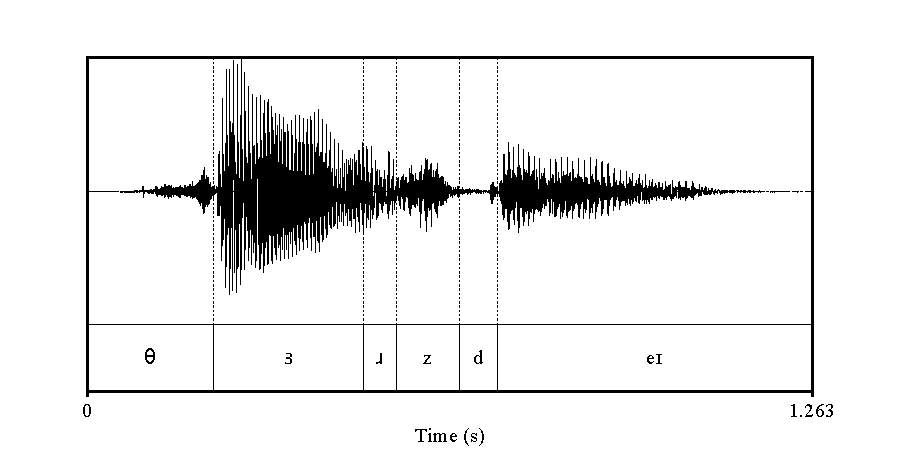
\includegraphics[width=\textwidth]{figures/spectrograms/thursday-spectrum}
\caption{A waveform for \exsent{Thursday}.}
\label{fig:waveform}
\end{figure}
  

The \keyword{pitch} of a sound -- how high or low it is -- provides
additional information, especially for vowels.  Speech is composed of
different frequencies all at once (due to the way sound reverberates
in the vocal tract).  The \keyword{fundamental frequency} F0 is also known as the pitch.  Absolute pitch varies across humans depending on the size of their vocal tract.  Relative variations in pitch can distinguishes tones in languages such as Chinese, where the pitch contour of a syllable distinguishes word meaning; rising pitch can indicate yes-no questions in English.  On top of pitch,  other higher-frequency \keywordAs{overtones}{overtone}, also known as \keyword{formants}, give unique character to each vowel and convey information about the position of the tongue in the mouth as it is articulated. The formant F1 corresponds to tongue height in the mouth, while F2 reflects its front/back position.

Finally, we can analyze spoken language using a \keyword{spectrogram},
which is a graph to represent the frequencies of speech ($y$-axis) over
time ($x$-axis).  As we can see in Figure~\ref{fig:spectrogram}, each
sound is a complex unit made of different frequencies.  In fact, what
we observe in a spectrogram will help us the most in automatically
determining what sound was uttered, which we turn to next.

\begin{figure}
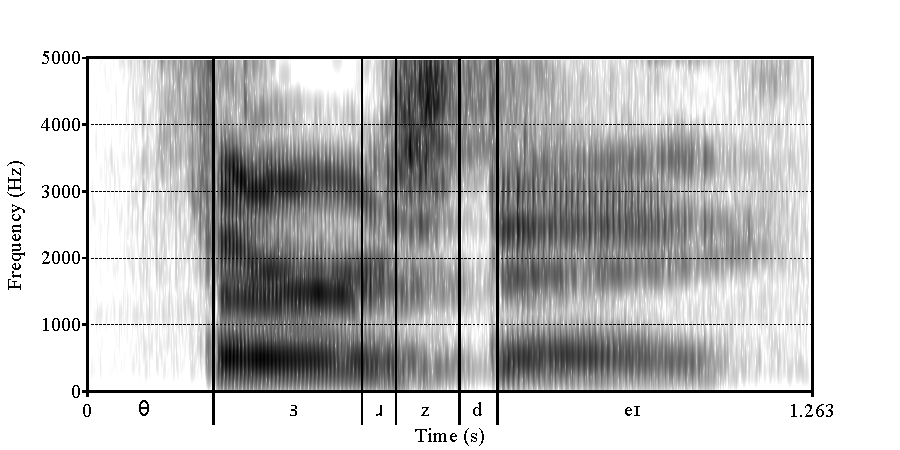
\includegraphics[width=\textwidth]{figures/spectrograms/thursday}
\caption{A spectrogram for \exsent{Thursday}.}
\label{fig:spectrogram}
\end{figure}

\subsection{Measuring speech}

A spectrogram has various measurable properties which tell us what the
sounds are.  The Under the Hood box on \emph{Reading a
  spectrogram} provides more details, but we will sketch a few general
properties here.  When looking at
a spectrogram, you should ask:

\begin{enumerate}
\item How dark is the picture?
  
  This tells us how loud each sound is and is measured in decibels.
  Different sounds differ in their loudness, including some sounds --
  such as {[d]} -- which involve a moment of complete silence.
  Compare [θ] and {[z]} in
  Figure~\ref{fig:spectrogram} showing that {[z]} is louder than [θ].  These are both fricative sounds, meaning that the air is channelled through a narrow passage in the mouth without stopping, but [θ] is voiceless (the vocal cords aren't vibrating) whereas {[z]} is voiced (with vibrating vocal cords) and thus sounds louder.

  
\item Where are the lines the darkest?
  
  The darkest lines tell us which frequencies (measured in hertz) are
  the loudest and the most important for determining the sound.  Each
  vowel has roughly three prominent frequency bands, and the vowels
  are distinguished by these bands.  For voiced sounds, we typically
  also see a low dark band.

\item How do these dark lines change?
  
  One last point involves how the frequencies change over time.  When
  we have stop consonants like {[t]} or {[k]}, there
  appears to be nothing in the spectrogram by which we can distinguish
  the sounds, and yet we make
  the distinction quite easily.  It turns out that the transitions of
  the vowel bands before and after the consonant are unique.

\end{enumerate}
\largerpage
It is these measurements which represent speech on the computer.  In
other words, to a computer, speech is nothing but a sequence of
various numerical measurements.  
After we discuss reading a spectrogram, we will delve into turning
these measurements of speech into text.



\begin{tblsfilledsymbol}{\underthehoodsubsection{Reading a spectrogram}}{glass}
\begin{underthehood}
% \vspace*{-\baselineskip}
The first thing to note about reading a spectrogram is that the word
boundaries are not at all clear-cut.  As mentioned before, there are
no pauses between words.  To know what a word is, what is needed is
information about the structure of the language we are looking at.
Consider, for example, hearing a string in a foreign language such as
\exsent{skarandashom}.  Can you tell where the word boundary is?  If
you speak Russian (and understand the transliteration from Cyrillic),
you might recognize the break between \exsent{s} (`with') and
\exsent{karandashom} (`(a) pencil').  Otherwise, you probably did not
know the boundaries.

But what about the individual sounds?  Let us start with the different
kinds of consonants.  When discussing articulatory properties of
speech, we distinguished the manner of articulation -- how air is
passed through the channel -- and it turns out that sounds with similar
manners have commonalities in their acoustic properties.  We will
examine three kinds of consonants: fricatives, nasals, and stops.
For each type of consonant, we will give a brief articulatory
description and then the acoustic distinctions that make it prominent.

We start our analysis with \keywordAs{fricatives}{fricative} -- in English, these include
{[f]} (\exword{f} in \exword{fist}, \exword{ph} in \exword{photo}), {[v]} (\exword{v} in \exword{vote}), {[s]}, {[z]},
[θ] (\exword{th} in \exword{thigh}), [ð]
(\exword{th} in \exword{thy}), [ʃ] (\exword{sh} in
\exword{she}), and [ʒ] (the final sound of \exword{rouge}).
All of these involve air passing turbulently through the mouth: The
tongue raises close to a point of constriction in the mouth, but it
does not completely touch.  With this turbulent air, we will see a lot
of ``noise'' in the spectrogram.
It is not completely noise, however; you can look at where the shading
is darkest in order to tell the fricatives apart.  For example, {[s]} generally has its energy
concentrated in the higher frequencies (e.g., close to 5000 Hz), as
illustrated in this spectrogram for \exword{fuss} [fʌs]:

\begin{figure}[H]
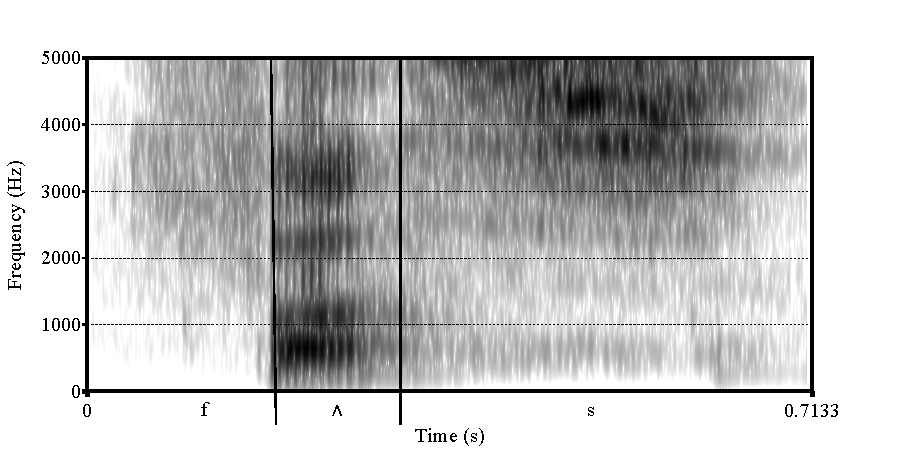
\includegraphics[width=\textwidth]{figures/spectrograms/fuss}
\caption{A spectrogram for \exsent{fuss}.}
\label{fig:fuss}
\end{figure}


On the other hand,
[ʃ] peaks lower (e.g., around 3500 Hz), and {[f]}
does not really have a prominent peak, as also shown in the figure.
The voiced sounds {[z]}, [ʒ], and {[v]}
pattern mostly like {[s]}, [ʃ], and {[f]},
respectively.  The main difference is that these sounds are voiced.
Voicing, which is the movement of vocal cords, causes there to be
low-frequency energy, though it is a bit hard to see precisely in the
spectrogram for the word \exsent{fuzz} [fʌz].
(Note, however, that the voicing difference co-occurs with a distinct
difference in the length of the vowel.)



\begin{figure}[H]
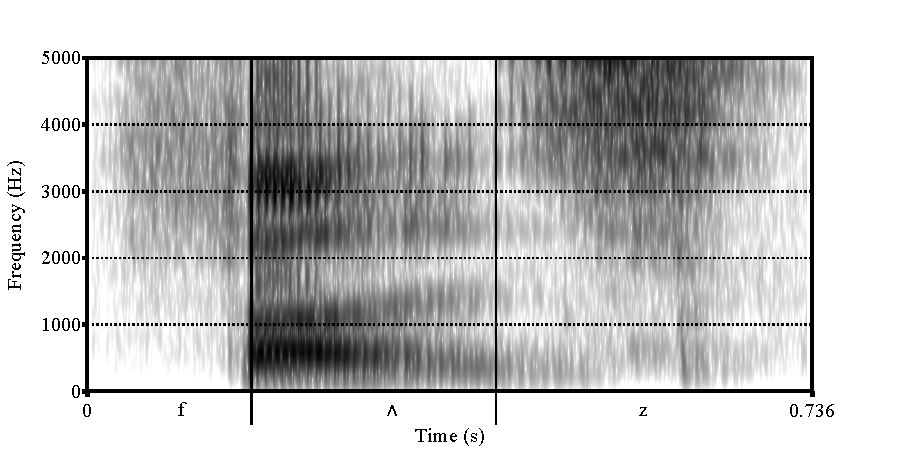
\includegraphics[width=.8\textwidth]{figures/spectrograms/fuzz}
\caption{A spectrogram for \exsent{fuzz}.}
\label{fig:fuzz}
\end{figure}

The next consonant type to look at is the set of \keywordAs{stop
  consonants}{stop consonant}, also called \emph{plosives}: {[p]} (\exword{p} in \exword{pad}), {[b]} (\exword{b} in \exword{boy}),
{[t]}, {[d]}, {[k]}, and {[g]} (\exword{g} in \exword{go}).  As
with fricatives, there are more stops in other languages.
What all of these sounds have in common is that, to make them, the
tongue makes a complete closure with part of the mouth.

But if there is a stoppage of air, then stops actually involve a lack
of sound.  So, how is it that we hear differences?  First of all, we
should note that stops are often accompanied by a burst of air -- what
is called \keyword{aspiration} -- which translates into noise (similar to
a fricative) in a spectrogram right after the stoppage.    We can see aspiration on the final /t/ in this spectrogram for \exword{deet} [dit].

\begin{figure}[H]
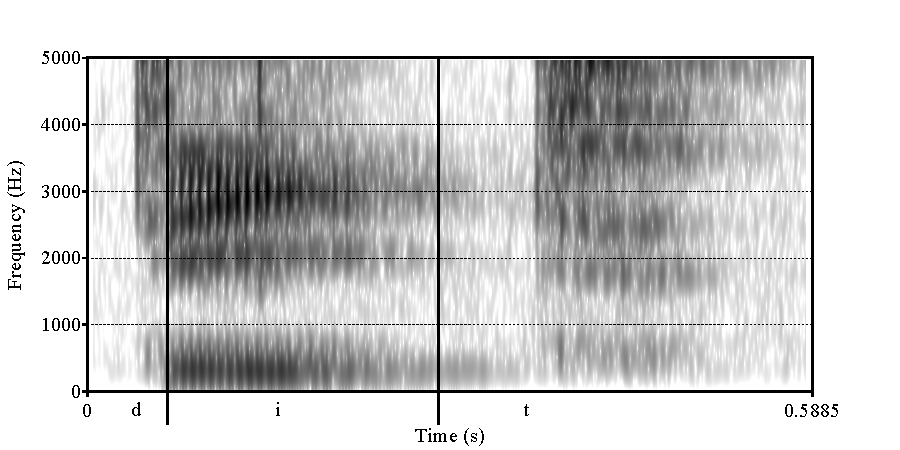
\includegraphics[width=.8\textwidth]{figures/spectrograms/deet}
\caption{A spectrogram for \exsent{deet}.}
\label{fig:deet}
\end{figure}

Second, more importantly, the way we hear a distinct stop
sound -- e.g., {[t]} vs. {[k]} -- is in the surrounding
vowels.  The vowels surrounding a consonant transition into the stop
and then out of it again, i.e., their formants (see below) move up or
down, depending on the consonant. 


We can now turn to \keywordAs{vowels}{vowel}, which can be difficult
to tell apart.  In articulation, a key aspect of vowels is
where in the mouth the tongue is raised: front, middle, or back.  We
can also talk about vowel height: If the tongue is raised high, low,
or somewhere in between.  Some of the vowels in English are given in
Table~\ref{tab:vowels}: {[i]} (\exword{beet}), [ɛ]
(\exword{bet}), [æ] (\exword{bat}), [ə] (the
\exword{a} in \exword{sofa}), {[u]} (\exword{boot}),
{[ow]} (\exword{boat}), and [ɑ] (the \exword{a} in
\exword{father}). 

\begin{table}[H]
\begin{tabular}{lccc}
\lsptoprule
     & Front         & Middle      & Back \\
High & {i}   &             & {u} \\
Mid  & ɛ   & ə & {ow} \\
Low  & æ &             & ɑ \\
\lspbottomrule
\end{tabular}
\caption{Some of the major vowels in English.}
\label{tab:vowels}
\end{table}

Vowels are generally distinguished by their three bands (stripes) of
frequencies: These are the vowel \keywordAs{formants}{formant}. We refer to these
as F1, F2, and F3.  Conveniently, there is a nearly direct
correspondence between the formant values and the location of the
tongue in the mouth.  F1 represents tongue height: The higher the F1 value, the lower the tongue
is.  F2 represents tongue front/backness: The higher the F2 value, the further forward in the mouth the tongue is.   The top (third) band, F3, reflects information about lip rounding and co-articulation of the consonant [{\textturnr}].

 In the spectrogram for \exword{deet},
for example, the {[i]} in \exsent{deet} has a low F1 band and
a high F2, representing the fact that it is a high, front vowel.

By measuring the formants F1 and F2, it is not just possible to distinguish between different vowels, but also to measure the accents (the position of the tongue in the mouth) of different people who are pronouncing the same vowel.  The linguistic subfield of \keyword{sociophonetics} uses such measurements to quantify how accents vary across people, regions, and time.

\end{underthehood}
\end{tblsfilledsymbol}


\subsection{Relating written and spoken language}

Having explored how both writing and sounds are represented digitally, we turn to the task of relating one to the other.    Automatic speech recognition (ASR) maps speech to text, and text-to-speech synthesis (TTS) maps text into sound.
  
Automatic speech recognition is the process by which a computer
converts a speech signal to text.  Such systems are enormously
practical, allowing for automatic transcription of podcasts and video calls, real-time dictation of note-taking, spoken conversations with digital assistants, and so on.

In general, ASR systems go through three steps.  First, speech is
digitally sampled, as was discussed above.  As this converts
continuous speech into a discrete representation, this will naturally
involve \keyword{information loss}.  Secondly, the speech samples are
converted into measurable units, as was also discussed above; this is
referred to as \keyword{acoustic signal processing}.  Here, the
digital samples are converted into, among other things, recognizable
frequencies, giving the computer a representation of speech to work
with.  These frequencies are used for the third step, the recognition
of sounds, groups of sounds, and words.  The frequencies can be used
to identify speech sounds, but, as we discussed before, the
interpretation of a given frequency is often ambiguous, since
different people speak differently.  For example, a {[t]}
might sound like a {[d]}.  The system will have to choose the most likely interpretation of an indeterminate sound by leveraging statistics about what people are most likely to say.


Given these basics, there are different kinds of ASR systems.  
\keywordAs{Speaker-dependent}{speaker-dependent} systems work for a
single speaker, whereas \keyword{speaker-independent} work for any
speaker of a given variety of a language, e.g., American English.
Given the range of pronunciations across different people,
speaker-dependent systems are clearly more accurate.  This is why
there are also \keyword{speaker-adaptive} systems, which start out as
independent systems but adapt over time to a single speaker in order to
improve accuracy.


The reverse process of automatic speech recognition is \keyword{text-to-speech}
(TTS) synthesis, which converts words into speech.  This might seem
like is a trivial task: Couldn't we simply record a voice saying
phrases or words and then play back those words in the appropriate
order?

While this might work for talking toy dolls, when we deal with
technology such as dialog systems (see \chapref{ch:dialog-systems}), the computer system generates
written sentences which need to be synthesized on the fly.  Thus, we
have to be able to break the text down into smaller units that can be
converted into speech.  This is challenging, given that writing system
representations are often phonetically ambiguous.

  

The main idea behind speech generation is to adjust the values of the
frequencies, the loudness, and other such properties, to produce the correct
sounds.  Since we know what frequencies correspond to which vowels,
for example, we can play those frequencies to make it sound like the
right vowel.  Of course, as we mentioned before, sounds are always
different, across time and across speakers.  Historically, one simple way to help in the
process of generating speech is to use a database of speech and to
use \keywordAs{diphones}{diphone}, i.e., two-sound segments, to generate new
utterances.  The contextual information found in diphones is useful because sounds are pronounced differently depending upon the neighboring sounds.

While these technologies are enormously useful and fascinating, they deserve textbooks in their own right. Moving forward, we set speech aside and focus on text.

\section{Consequences}

Spoken/signed language allows us to communicate face-to-face, while written language allows us to communicate across space and time.  Digital writing allows us communicate with more people around the world than ever before, and machine-readable text provides data for various applications of language technology to be explored throughout the book.


Foreshadowing some larger themes, this chapter also illustrates how linguistic information (writing, sounds) can be interpreted qualitatively by humans but must be represented quantitatively (in bits, in hertz) on a computer.  Throughout the book, we will encounter more ways that computers can quantify language.  

Moreover, this chapter shows how text represents some, but not all, of the information conveyed by language.  A word is a pairing of sound and meaning, but a phonetic writing system such as our Latin alphabet represents only  sounds.  While a human knows the meaning independently, what semantic information is available to a computer which has access only to the textual representation of  sound?  The rest of the book will explore how computers, without access to the outside world or the mental representations available to humans, can approximate meaning.

% also the idea that words have both sound and meaning and that a writing system does not necessarily represent meaning; have to know that independently (how would a computer know it?)


%\begin{underthehood}
%\underthehoodsubsection{Language modeling for automatic speech recognition}
%\label{uth:asr-modeling}

%Although we have talked a great deal about the acoustic information that goes into speech recognition, acoustics is not the only source of information. For example, if the system already recognized the previous words correctly, then knowing these correct words could help us get the next word correct.

%Consider what happens when a system thinks it has recognized a syllable sounding like {[ki]}.  Without knowing anything about the context, the most likely word is \exsent{key}, but, given all the fluctuations in how speakers say a word, this could also be \exsent{Guy}, \exsent{keep}, \exsent{keyed}, \exsent{keen}, or even the latter part of \exsent{ski}.

%The problem is that all of these are plausible words or parts of words for that sound: sounds like {[g]} and {[k]} are easily confused; final consonants can be dropped; and the preceding sound may or may not be a part of this word (e.g., \exsent{his skis} and \exsent{his keys} sound nearly identical).  While certain facts about pronunciation are useful -- e.g., the likelihood of dropping a {[p]} at the end of a word -- what we really need is some notion of the wider context.

%Specifically, knowing something about the previous word can help. Consider if the previous word was recognized as \exsent{is}: all of a sudden, \exsent{keep} and \exsent{key} are less likely.  If the previous word was \exsent{the}, we have a different set of best candidates: in this case (assuming no previous \exword{s} sound), \exsent{key} is probably the best choice.  The intuition is that facts about the (previous) context should give us better word guesses.  Now, the question is: how can we capture this intuition in a computationally practical way?

%One concept that will help here and in the chapters to come is that of an \keyword{$n$-gram}, a stretch of text $n$ units (here: words) long. We can use $n$-grams to approximate language, as they say something about language, without capturing the entire structure, and are a very efficient technique for language processing.  Finding, for example, every two-word sequence in a text is quick and easy.

%$N$-grams help a variety of natural language processing (NLP) applications, including the task we are interested in, namely \keyword{word prediction}.  We can look at the previous words (i.e., the previous $n-1$ words) to predict the next word.  If we use 3-grams, or \keywordAs{trigrams}{trigram}, we will use the previous two words to predict the current word.

%Let us start with a phrase like \exsent{I dreamed I saw the knights  in}, the first seven words of the Neil Young song \mediatitle{After the  Gold Rush}.  Before we get into technical points, what do you think the next word is?  Even if they have never heard the song, many people will answer with \exsent{shining} or \exsent{armor} (the correct word, in this case).  In fact, if you had seen the phrase \exsent{knights   in} and were asked to predict the next word, your choices would likely be the same.  That is, we often only need two words to be able to say something useful about the next word.  (Of course, homophones, such as \exword{nights in}, as in The Moody Blues' \mediatitle{Nights in White  Satin} could cause a problem here.)

%We will return to this point in a moment, but, first, let us lay out the more mathematical properties of this situation.  In order to make sense of $n$-gram information, we want to know how likely an $n$-gram is.  Thus, we will use probabilities.  A \keyword{probability} captures the likelihood of something happening.  For example, maybe the probability of seeing someone carrying an open umbrella on a given college campus is 10\%.

%What we will actually need to do is to look at the probability of one event if we know something about another related event.  Let us walk through an example to see what this means.  Consider the probability of seeing a professor walking across the Ohio State campus carrying an open umbrella. The weather in Ohio is usually quite good, so this probability is probably low, e.g., 10\%.  But, if we know that it has been raining for the last three hours, then our estimate of the probability increases markedly. In the language of probability, we call the fact that it has been raining for the last three hours the \keyword{conditioning event}, and the fact that we actually observe the professor with the umbrella the \keyword{conditioned event}.  The idea of using conditional probabilities here is to take account of the fact that rain influences the behavior of professors. Of course, this tendency cannot be totally relied on, because professors are notoriously erratic and insensitive to their environment. But, on average, it remains true that rain will increase the rate with which umbrellas are present and open.

%Similarly, the idea of language modeling is to form conditional probabilities that reflect our judgment about the influence that the previous words will have on their successors.  In the case of \exsent{I dreamed I saw the knights in}, the conditional probability we are interested in is the probability of the next word given that we have already seen \exsent{I dreamed I saw the knights in}.

%Mathematically, we denote conditional probabilities by using a $|$ symbol.  We can read something like $P(A|B)$ as ``the probability of A given B.''  In this case, if we want to know the likelihood of \exsent{armor} being the next word, we are interested in $P(armor|I$ $dreamed$ $I$ $saw$ $the$ $knights$ $in)$.

%But this seems like a strange probability.  Do we really need 7 words to predict the eighth one?  Most of these words are unimportant for predicting the next word.  Furthermore, if we have to do word prediction with a computational system, it will take us an enormous amount of memory to store all these 8-grams, or 10-grams, or 25-grams, or however long.

%The solution for this situation is simple: we use our intuition from before -- that we only need a few words to accurately predict the next word -- and approximate this probability.  A \keyword{trigram} approximation for this string is in (\ref{ex:tri-approx}), where $\approx$ means ``is approximately equal to.''  This says that we should only look at the previous two words to predict the next word.

%\begin{exe}
%  \ex\label{ex:tri-approx} $P(armor|I$ $dreamed$ $...$ $knights$ $in) \approx
%  P(armor|knights$ $in)$
%\end{exe}

%Common approximations are to use \keywordAs{bigrams}{bigram} ($n=2$) or trigrams ($n=3$).  The choice of how long an $n$-gram should be is a tradeoff between robustness and accuracy.  The shorter the $n$-gram, the more examples we can find -- after all, for a string of four words there is a single 4-gram, but two 3-grams, three 2-grams and four 1-grams (or \keywordAs{unigrams}{unigram}). So the chance of finding the same bigram twice in a text is greater than that of finding the same trigram twice. The lower the value of $n$, the more instances of such $n$-grams we find, meaning that a system will be able to account for more situations and thus be more \keyword{robust}.

%One remaining question is: what do we do when we encounter a trigram we have never seen before?  For example, someone might utter \exsent{eat loaves}, and we have never seen this phrase before, so we are not sure what the next word should be. While we will not delve into this topic too deeply, systems employ techniques for dealing with unknown data, often called \keyword{smoothing}. One such technique is to \keyword{back off} to a shorter $n$-gram when the current one cannot be found.  For example, in this scenario, we would check all bigrams starting with \exsent{loaves} in order to predict the next word (e.g., \exword{of}).

%Continuing our \exsent{knights in armor} example, if the system is deciding between \exsent{armor}, \exsent{harmful}, and the two-word sequence \exsent{arm or}, an $n$-gram model as we have outlined should be able to tell us that \exsent{armor} is the preferred word.

% Recall also the similar example at the beginning of this section, namely trying to decide between \exsent{keen}, \exsent{key}, and \exsent{keyed}, among other choices.  When we put all this information together in a given context, one probability should outweigh another, as in (\ref{ex:need}).  Using these probabilities, the system's best guesses at speech sounds can be turned into sequences of real words.

%\begin{exe}
%  \ex\label{ex:need} $P(key|the) > P(keen|the) > P(keyed|the)$
%\end{exe}

% The concepts of using $n$-grams and probabilities will recur throughout this book, such as in the writers' aids section on using $n$-grams to assist with spelling correction, section~\ref{sec:n-gram-methods}, and in Under the Hood~\ref{sec:noisy-channel-model} in the machine translation chapter, where some of the theoretical underpinnings of using probabilities to recover information are given.

%\end{underthehood}


\begin{tblsfilledsymbol}{Checklist}{test}

\begin{itemize}
\item Describe different types of writing systems (with examples) and how they vary in
  their use of phonetic and semantic properties. 
  \item Explain the meaning of the rows and columns in the International Phonetics Alphabet for consonants.  Explain the organization of the vowel chart.
\item Discuss why it is possible for a language  to be written in several different writing systems, and what this shows about the relationship between the written and spoken forms of language.
\item Recognize that numbers can be represented in different ways, and 
understand how to convert between representations, especially
converting numbers between base 2 and base 10 representations.
\item Explain what Unicode is useful for and how the UTF-8 encoding
  scheme works.
\item Sketch how modern technology allows the acoustic properties of speech sounds to be measured, and 
know how to recognize some speech features by looking at spectrograms. 
\item Explain the tasks of automatic speech recognition and
  text-to-speech synthesis, and distinguish between speaker-dependent, speaker-independent, and speaker-adaptive approaches.
\end{itemize}

\end{tblsfilledsymbol}


\begin{tblsfilledsymbol}{Exercises}{pencil}

\begin{enumerate}

\item Using the distinctive features of language from the beginning of the chapter, discuss whether music, mathematics, programming languages, or body language can be considered ``language'' in Hockett's sense.



\item  Visit Omniglot\footnote{\url{https://omniglot.com}, accessed 2024-05-23.} and pick a
  syllabary.  Take a paragraph from a novel written in English and
  transliterate it into this syllabary.
  \begin{enumerate}
  \item What difficulties do you encounter?
  \item Is there any \emph{information loss} in your transliteration?
    If it were transliterated back into the Latin alphabet, what
    ambiguities would you find?
  \end{enumerate}
\item  Assume you've been given power to alter the Latin
  alphabet for the purposes of better writing down English words.
  \begin{enumerate}
  \item Keeping it as an alphabet, what would you change, add, or
    remove?  Why?
  \item Could you just use the IPA to write down English?  What
    problems might you encounter?  Would it be easier or harder for English speakers around the globe to communicate in writing?
  \item Could you convert the alphabet into a system similar to
    Hangeul for Korean?  How would it work?
  \item Assume you have to propose 100 words to be replaced by (logographic) emoji.  What types of words would you select for the first 100?
    Why?
  \end{enumerate}
\end{enumerate}

\begin{enumerate}
  \setcounter{enumi}{2} 

\item  As mentioned briefly, \emph{hexadecimal} numbers
  have 16 digits: 0-9 and then the letters A-F. They are commonly used
  in computing because they more compactly represent the numbers which
  are often used for bytes than binary numbers do.
  \begin{enumerate}
  \item Describe how hexadecimal numbers work, working through the
    base ten number 46 as an example.
  \item Describe a procedure for converting numbers from a binary
    (base two) to a hexadecimal (base sixteen) representation.
  \end{enumerate}
\item  Discuss the optimal way to design UTF-8, in terms of
  the average number of bytes per character and the number of users of
  a given writing system.
\end{enumerate}

\begin{enumerate}
\setcounter{enumi}{4}

\item  The speech waveforms and spectrograms shown in
  this chapter were produced using Praat, but there are other useful
  speech analysis software kits, such as Wavesurfer and VoiceSauce.

  \begin{enumerate}
  \item Explore one of these software packages and make yourself comfortable with using it.
  \item Pick your favorite book and record yourself reading the first
    sentence (or 20 words, whichever comes first).
  \item Record a friend saying the same thing.
  \item Compare and contrast spectrograms of your different spoken
    language examples, describing how what you see corresponds to what
    you both said and what the differences are.
  \end{enumerate}
\item  Explain why ASR is an irreversible process. Make
  reference to the concept of \emph{information loss} in your answer.

\end{enumerate}
\end{tblsfilledsymbol}

% \begin{enumerate}
% \setcounter{enumi}{6}




% \end{enumerate}

\begin{tblsfilledsymbol}{Further reading}{book}


Hockett's design features of language are pioneered in \citet{Hockett:1960}.

More information on writing systems, including various nice graphics,
can be gleaned from websites such as Omniglot\footnote{\url{https://omniglot.com}, accessed 2024-04-19.}.
Additionally, there are books on writing systems, such as
\citet{daniels:bright:96}.  \citet{sproat:00} offers a unique
treatment, which focuses on computational properties of writing
systems, and \citet{Sproat-11} extends the writing system discussion
to language technology and its impact on society. Both are highly
recommended.  Turning from writing systems to language, a thorough set
of information on the world's languages can be found in the Ethnologue
\citep{gordon:05}. For an accessible overview of topics related to
language and how language can be studied, check out the \mediatitle{Language Files}
\citep{LanguageFiles13}. As a reference book, you can find
comprehensive information in David Crystal's Encyclopedia of Language
\citep{Crystal-11}.

\citet{McCulloch:2020} explores the influence of the internet on language and writing, with detailed discussion of emoji.

For an introductory look at automatic speech recognition and language
modeling, the \citet{Jurafsky.Martin-09} textbook is a valuable
resource. 
%There are also papers such as \citet{madnani:09}, which provide nice overviews of language modeling, and you can check out practical toolkits, such as SRILM \citep{stolcke:02}, at \url{http://purl.org/lang-and-comp/srilm}.  
For a thorough
introduction to the field of phonetics, we recommend \citet{LadefogedJohnson:2014}. 

\end{tblsfilledsymbol}
